% Giữ mẫu Elsevier CAS hai cột của bản thảo gốc.
\PassOptionsToPackage{T5}{fontenc}
\documentclass[a4paper,fleqn]{cas-dc}

\usepackage[utf8]{inputenc}
\usepackage[T5]{fontenc}
\usepackage[vietnamese]{babel}
% Tương thích compiler XeTeX tích hợp; pdfLaTeX vẫn dùng khai báo gốc.
\ifdefined\DeclareUnicodeCharacter
\DeclareUnicodeCharacter{00D7}{\ensuremath{\times}}
\fi
\usepackage[numbers]{natbib}
\usepackage{amsmath,amssymb}
\usepackage{booktabs}
\usepackage{tabularx}
\usepackage{longtable}
\usepackage{array}
\usepackage{enumitem}
\usepackage{microtype}
\usepackage{hyperref}
\usepackage{xcolor}
\usepackage{graphicx}
% Phụ trợ v2; giữ nguyên CAS/T5/babel và các nhãn Việt hóa.
\graphicspath{{figures/}{./}}
\usepackage{tikz}
\usetikzlibrary{arrows.meta,positioning}
\usepackage{pgfplots}
\pgfplotsset{compat=1.18}
\newif\ifbranchB
\branchBfalse % Giữ nhánh B để tác giả duyệt; bật bằng branchBtrue.

\usepackage{algorithm}
\usepackage[noend]{algpseudocode}
\floatname{algorithm}{Thuật toán}
\algrenewcommand\algorithmicrequire{Đầu vào:}
\algrenewcommand\algorithmicensure{Đầu ra:}
\algrenewcommand\algorithmicfor{Với}
\algrenewcommand\algorithmicdo{thực hiện}
\algrenewcommand\algorithmicif{Nếu}
\algrenewcommand\algorithmicthen{thì}

\renewcommand{\abstractname}{Tóm tắt}
\renewcommand{\figurename}{Hình}
\renewcommand{\tablename}{Bảng}
\renewcommand{\refname}{Tài liệu tham khảo}
\renewcommand{\encodingdefault}{T5}
\AtBeginDocument{\fontencoding{T5}\selectfont}
% Nhánh XeTeX cho compiler tích hợp; pdfLaTeX giữ nguyên cơ chế T5 gốc.
\ifdefined\XeTeXversion
\usepackage{fontspec}
\setmainfont{texgyretermes-regular.otf}[BoldFont=texgyretermes-bold.otf,ItalicFont=texgyretermes-italic.otf,BoldItalicFont=texgyretermes-bolditalic.otf]
\setsansfont{texgyreheros-regular.otf}[BoldFont=texgyreheros-bold.otf,ItalicFont=texgyreheros-italic.otf,BoldItalicFont=texgyreheros-bolditalic.otf]
\setmonofont{texgyrecursor-regular.otf}
\renewcommand{\encodingdefault}{TU}
\AtBeginDocument{\fontencoding{TU}\selectfont}
\fi


% Chỉ Việt hóa nhãn; giữ kích thước và cấu trúc hộp của CAS 2.4.
\ExplSyntaxOn
\RenewDocumentEnvironment{keywords}{O{Từ~khóa}}
{
  \tex_global:D \tex_setbox:D \g_stm_key_box = \vtop \bgroup
  \hsize=.25\textwidth
  \cs_set:Npn \sep: { \par }
  \cs_set_eq:NN \sep \sep:
  \parindent=0pt
  THÔNG~TIN~BÀI~BÁO \par \skip_vertical:n { -3pt }
  \rule{.25\textwidth}{.2pt}\par\footnotesize
  \noindent \textit{#1}: \par
}{\egroup}
\ExplSyntaxOff

% [override] Bỏ "Preprint submitted to Elsevier" ở footer trang đầu; chỉ hiện tên tác giả.
\ExplSyntaxOn
\cs_set:Npn \__first_footerline:
{
  \group_begin:
  \small \sffamily
  \ifnum\theblind>0\relax\else \__short_authors: \fi
  \group_end:
}
\ExplSyntaxOff

% Lệnh riêng của bản thảo này
\newcommand{\nodata}[1]{\textcolor{red}{[CHƯA CÓ SỐ: #1]}}
\newcommand{\Ntau}{N_{\tau}}
% Giữ hình/bảng gần chỗ được nhắc: chặn trôi qua ranh giới mục và nới các tham số đặt float
\usepackage{placeins}
\usepackage{adjustbox}
\usepackage{float}
\usepackage{capt-of}
\renewcommand{\topfraction}{0.9}\renewcommand{\bottomfraction}{0.8}\renewcommand{\textfraction}{0.07}
\renewcommand{\floatpagefraction}{0.6}\renewcommand{\dbltopfraction}{0.9}\renewcommand{\dblfloatpagefraction}{0.6}
\setcounter{topnumber}{4}\setcounter{bottomnumber}{2}\setcounter{totalnumber}{8}\setcounter{dbltopnumber}{4}

\begin{document}
\let\WriteBookmarks\relax
\def\floatpagepagefraction{1}
\def\textpagefraction{.001}
\shorttitle{Số ứng viên trước NMS và độ trễ}
\shortauthors{Phạm Tuấn Anh và Mai Quốc Bảo}
\title[mode=title]{Số lượng ứng viên trước NMS có dự đoán được độ trễ của bộ phát hiện không? Một nghiên cứu đo lường trên lõi CPU được ghim và một nghiên cứu tình huống về tối ưu hóa patch}
\author[1]{Phạm Tuấn Anh}
\ead{anh25807700004@hutech.edu.vn}
\author[1]{Mai Quốc Bảo}
\ead{bao2580770008@hutech.edu.vn}
\cortext[cor1]{Tác giả liên hệ: Đinh Phương Nam. Email: dp.nam@hutech.edu.vn.}
\nonumnote{Giảng viên hướng dẫn: Đinh Phương Nam, Trường Đại học Công nghệ Thành phố Hồ Chí Minh (HUTECH). Email: dp.nam@hutech.edu.vn.}
\affiliation[1]{organization={Trường Đại học Công nghệ Thành phố Hồ Chí Minh (HUTECH)},
city={Thành phố Hồ Chí Minh},country={Việt Nam}}

\begin{abstract}
Các tấn công độ trễ lên bộ phát hiện đối tượng thường cực đại hóa số ứng viên đi vào bước loại bỏ không cực đại (NMS), $\Ntau$, với giả định rằng ứng viên càng nhiều thì pipeline càng chậm. Chúng tôi kiểm tra giả định này như một bài toán đo lường, bằng một giao thức có ghim lõi CPU được kiểm chứng dưới tải, đo từng công đoạn và hiệu chuẩn A/A để nêu hiệu ứng nhỏ nhất phát hiện được (MDE) của mọi phép so sánh, trên một CPU laptop. Ba phát hiện chính. Thứ nhất, khi tiêm $10^2$ đến $10^4$ ứng viên tổng hợp, độ trễ NMS tăng từ 4 đến 1360 lần tùy cách cài đặt và hình học, và giới hạn top-300 loại bỏ phần lớn mức tăng. Thứ hai, tỷ số toàn trình được dự đoán tốt bởi một mô hình kiểu Amdahl không có tham số khớp, chỉ dùng đường cong tiêm và thời gian của ảnh sạch: sai số trung vị 1,2\% trên 156 ô tiêm vào toàn pipeline, và ngưỡng ứng viên cần để thấy toàn trình chậm đi trùng với phép đo ở 35 trên 48 ô. Thứ ba, trên các tấn công toàn ảnh thật (Overload, Phantom Sponges) đẩy $\Ntau$ lên khoảng 5000 (gấp khoảng 350 lần ảnh sạch), toàn trình chỉ tăng 3\%; mô hình dự đoán đạt quy tắc định trước ở 3 trên 6 ô và hụt vì đường cong tổng hợp đánh giá quá cao chi phí NMS của ứng viên thật. Một bộ tối ưu patch bằng thuật toán di truyền không làm tăng $\Ntau$ và không vượt tìm kiếm ngẫu nhiên. Các kết quả giới hạn ở suy luận trên CPU một lõi, nơi lan truyền thuận chiếm phần lớn thời gian; thiết bị có bộ tăng tốc chưa được đo.
\end{abstract}

\begin{keywords}[Từ khóa]
phát hiện đối tượng \sep loại bỏ không cực đại (NMS) \sep đo độ trễ \sep patch đối kháng \sep tối ưu hộp xám \sep thuật toán di truyền \sep tính sẵn sàng
\end{keywords}
\maketitle

\section{Giới thiệu}
Các bộ phát hiện đối tượng dùng NMS tiêu tốn một phần thời gian của mỗi khung hình vào việc loại bỏ các hộp ứng viên chồng lấn nhau. Vì chi phí của NMS tham lam phụ thuộc vào số ứng viên vượt ngưỡng điểm, một hướng nghiên cứu chế tác đầu vào sao cho số này tăng lên để làm chậm quá trình phát hiện \cite{phantom2023,overload2024}, mở rộng ý tưởng tấn công năng lượng--độ trễ trên mạng nơ-ron \cite{shumailov2021sponge}. Trong các công trình này, số ứng viên $\Ntau$ vừa là đại lượng được cực đại hóa vừa là lời giải thích cho mức chậm quan sát được. Vai trò thứ hai là một khẳng định thực nghiệm: chi phí NMS còn phụ thuộc vào cách cài đặt và vào cách các hộp chồng lấn, và NMS chỉ là một công đoạn của pipeline. EVADE đã cho thấy các tấn công độ trễ NMS thường không đạt mức như công bố khi chuyển sang cấu hình triển khai \cite{evade2025}. Bài này không đánh giá lại các tấn công; nó kiểm tra trực tiếp đại lượng mà chúng tối ưu và xây một mô hình định lượng cho biết khi nào $\Ntau$ chuyển thành độ trễ toàn trình.

Chúng tôi đặt bốn câu hỏi.
\begin{description}[leftmargin=2.5em,labelwidth=2.2em,itemsep=2pt]
\item[Q1] Khi các ứng viên được kiểm soát, độ trễ NMS phụ thuộc vào $\Ntau$, cách cài đặt NMS, hình học hộp và giới hạn top-$k$ như thế nào trong khoảng $10^2$ đến $10^4$ ứng viên?
\item[Q2] Cần bao nhiêu ứng viên để độ trễ toàn trình tăng vượt sàn nhiễu, và một mô hình kiểu Amdahl có dự đoán được ngưỡng đó không?
\item[Q3] Trên các tập ứng viên thật do tấn công tạo ra, kể cả các tấn công toàn ảnh đẩy $\Ntau$ lên hàng nghìn, độ trễ toàn trình thay đổi bao nhiêu và mô hình có dự đoán đúng không?
\item[Q4] Một bộ tối ưu patch kiểu thuật toán di truyền, với hàm mục tiêu chỉ dựa trên $\Ntau$ và điểm số, có tạo ra mức tăng $\Ntau$ hay độ trễ nào không?
\end{description}

\paragraph{Đóng góp.}
(i) Một giao thức đo độ trễ pipeline có ghim lõi được kiểm chứng dưới tải, đo từng công đoạn, hiệu chuẩn A/A và đăng ký trước các endpoint. (ii) Một đối chứng dương tiêm ứng viên tổng hợp vào chính pipeline, lập bản đồ độ trễ NMS theo $\Ntau$, cách cài đặt, hình học và giới hạn top-$k$, và đo ngưỡng $N^{*}$ ở mức toàn trình. (iii) Một mô hình kiểu Amdahl không tham số khớp, $R \approx 1 + \Delta t_{\mathrm{NMS}}(\Ntau, \text{cài đặt}, \text{hình học})/t_{\mathrm{total}}$, được kiểm trên phép tiêm toàn pipeline và kiểm tiến cứu trên các tấn công thật, kèm phân tích chỗ mô hình hụt. (iv) Các phép đo dưới giao thức này trên các tấn công toàn ảnh đã công bố (dạng điều chỉnh) và trên một bộ tối ưu patch, cho thấy mức tăng toàn trình thực tế trên CPU nhỏ hơn nhiều so với mức tăng của $\Ntau$.

\paragraph{Bố cục.}
Mục~\ref{sec:related} điểm lại công trình liên quan; Mục~\ref{sec:formal} hình thức hóa $\Ntau$, nêu mô hình chi phí và mô hình kiểu Amdahl; Mục~\ref{sec:protocol} mô tả giao thức và các thí nghiệm; Mục~\ref{sec:results} báo cáo kết quả theo thứ tự đối chứng dương, mô hình dự đoán, tấn công thật và nghiên cứu tình huống; Mục~\ref{sec:discussion} thảo luận; Mục~\ref{sec:threats} nêu các giới hạn; Mục~\ref{sec:conclusion} kết luận.

\section{Công trình liên quan}
\label{sec:related}
\subsection{Dòng tấn công cạn kiệt tài nguyên và vị trí của Sponge Patch}
Tấn công nhắm tính sẵn sàng xem hiệu quả tính toán là một bề mặt tấn công riêng bên cạnh tính đúng đắn: đầu vào được tối ưu để tăng khối lượng tính toán và kéo dài thời gian xử lý mà không nhất thiết làm sai nhãn. Các sponge example làm tăng năng lượng hoặc độ trễ của một mạng bằng các đầu vào được chế tác \cite{shumailov2021sponge}, và NICGSlowDown minh họa nguyên lý này trên mô hình sinh chú thích ảnh bằng cách kéo dài chuỗi sinh \cite{nicgslowdown2022}. Với bộ phát hiện, điểm phình tính toán đặc trưng là bước khử trùng lặp NMS, chi phí tăng theo số hộp ứng viên. Phantom Sponges biến quan sát này thành tấn công độ trễ: tối ưu nhiễu toàn ảnh hộp trắng để số hộp sống sót sau ngưỡng tăng vọt, buộc NMS chạy lâu hơn và làm chậm bộ phát hiện thời gian thực \cite{phantom2023}. Overload theo cùng hướng và nhấn mạnh bối cảnh thiết bị biên, nơi một lần suy luận kéo dài đủ phá vỡ thời hạn \cite{overload2024}. SlowTrack chuyển mục tiêu từ một khung hình sang toàn chuỗi tri giác của xe tự lái, cho thấy độ trễ tích lũy mới là đại lượng gây hại ở mức hệ thống \cite{slowtrack2024}.

Song song, dòng miếng dán đối kháng cục bộ chủ yếu nhắm làm sai (ẩn hoặc đánh lừa) thay vì làm chậm: các khảo sát và phòng thủ miếng dán gần đây tập trung vào đánh giá nhất quán, khử nhiễu và huấn luyện đối kháng \cite{apde2025,pbcat2025}, còn hướng tối ưu vị trí và tính hợp lệ vật lý mở rộng khả năng che giấu của miếng dán \cite{iap2025,badpatch2025}. Hai dòng, cạn kiệt tài nguyên (thường nhiễu toàn ảnh hộp trắng) và miếng dán cục bộ (thường nhắm làm sai), gần như tách biệt về mục tiêu. Sponge Patch nằm ở giao của hai dòng và chọn một điểm quyền truy cập khác (Bảng~\ref{tab:related}): một miếng dán cục bộ, không cần gradient, chỉ dùng phản hồi điểm tin cậy trước NMS làm tín hiệu tối ưu, với mục tiêu khảo sát, chưa khẳng định, khả năng gây tải NMS. Vì khác mô hình đe dọa và bề mặt tấn công, con số của những công trình trên không so trực tiếp được với kết quả của nhóm; chúng là mốc định tính để định vị giả thuyết và lý giải vì sao bài tách riêng bốn đại lượng đo.

\subsection{Tấn công và phòng thủ đối với tính sẵn sàng}
Underload nhấn mạnh mối liên hệ giữa hành vi đối kháng và năng lực phần cứng, đồng thời sử dụng huấn luyện đối kháng có chú ý nền để cân bằng hiệu năng sạch và khả năng xử lý thời gian thực \cite{underload2025}. Hướng này trực tiếp bảo vệ dịch vụ nhưng đòi hỏi truy cập và cập nhật mô hình. EVADE kiểm tra tính thực dụng dưới nhiều thiết bị và định dạng thay vì chỉ tối ưu một đại lượng đại diện \cite{evade2025}: nó định nghĩa một khung đánh giá, áp dụng cho các tấn công độ trễ NMS hiện có trên nhiều nền tảng phần cứng, định dạng mô hình và thiết lập lượng tử hóa, báo cáo rằng các tấn công này không tạo ra mức tăng độ trễ như đã công bố, không chuyển sang mô hình khác, và mức tăng vẫn nằm trong yêu cầu độ trễ của tác vụ phía sau. Bài này tiếp nhận yêu cầu đo thực thi của hướng đánh giá đó; chưa chứng minh một cơ chế phòng thủ tương đương Underload.

Tấn công bit-flip làm tăng độ trễ bộ phát hiện có mô hình đe dọa khác: can thiệp tham số qua lỗi bit, thay vì giữ trọng số cố định và chỉ sửa đầu vào \cite{bitflip2025}. TrackFlood khảo sát việc chuyển bề mặt tấn công từ bộ phát hiện không NMS sang bộ theo dõi \cite{trackflood2026}. Event Burst Trigger xem xét backdoor tính sẵn sàng trên bộ phát hiện dùng mạng nơ-ron xung \cite{eventburst2026}. Hai tài liệu sau được trích theo bản arXiv; chúng tôi không dùng trạng thái công bố chưa xác minh để coi chúng là bằng chứng đã được tái lập. Các hướng này cho thấy loại bỏ NMS khỏi bộ phát hiện không đồng nghĩa loại bỏ mọi chi phí phụ thuộc nội dung của hệ thống hoàn chỉnh.

\subsection{Đánh giá và phòng thủ miếng dán}
Benchmark APDE đặt trọng tâm vào đánh giá nhất quán giữa nhiều tấn công, bộ phát hiện và chỉ số; kết quả cho thấy phát hiện được patch không tự đồng nghĩa phục hồi vật thể bị tấn công \cite{apde2025}. PBCAT kết hợp miếng dán cục bộ với nhiễu toàn ảnh trong huấn luyện đối kháng để mở rộng phạm vi phòng thủ đối với các tấn công vật lý \cite{pbcat2025}. ODDR, DiffPAD và một hướng bộ phát hiện patch có khả năng giải thích khảo sát các cơ chế tiền xử lý hoặc nhận diện vùng nhiễu khác nhau \cite{oddr2025,diffpad2025,unifiedpatchdet2025}. Vì thêm công đoạn có thể làm tăng độ trễ hoặc xóa thông tin hữu ích, việc đánh giá phòng thủ trong bài này giữ cả AP/AR lẫn chi phí hậu xử lý. AntiStyler và TRACE tiếp tục khảo sát phòng thủ bộ phát hiện trước miếng dán và cách tinh chỉnh đối kháng nhằm giảm ảnh hưởng của yếu tố gây nhiễu \cite{antistyler2026,trace2026}; những công trình này là đối chiếu cho nghiên cứu phòng thủ.

\subsection{Tối ưu vị trí và tính hợp lệ vật lý}
IAP kết hợp định vị nhận biết khả năng bị nhìn thấy với tối ưu nhiễu để tạo miếng dán khó nhận biết \cite{iap2025}. Một hướng nghiên cứu khác xem xét hình dạng phổ quát của patch đặt từ xa đối với bộ phát hiện CNN \cite{remotepatch2025}. Các cách tối ưu vị trí và hình dạng này là cơ sở đối chiếu cho heuristic Laplacian: heuristic của nhóm có chi phí đơn giản và không cần gradient, nhưng không phải mô hình hóa đầy đủ độ nhạy của bộ phát hiện hoặc khả năng quan sát vật lý. BadPatch sử dụng mô hình khuếch tán để tạo miếng dán vật lý và cung cấp bối cảnh dữ liệu áo đối kháng \cite{badpatch2025}. GRAC và hướng tạo camouflage đa góc nhìn bằng 3D Gaussian Splatting chú ý tới sự khác nhau giữa góc nhìn, ánh sáng và quy trình dựng hình \cite{grac2025,gs3dcamo2025}. Những yếu tố đó vượt ra ngoài phân phối xoay, màu, mờ và nhiễu ảnh mà Sponge Patch hiện dùng. Các công trình về quần áo đối kháng nhiệt--thị giác mở rộng sang cảm biến đa phương thức \cite{rgbt2026,thermal2026}; nghiên cứu hiện tại chỉ dùng ảnh RGB và không suy rộng kết quả sang cảm biến nhiệt. Patch đối kháng nói chung là các nhiễu loạn cục bộ, không phụ thuộc ảnh \cite{brown2017patch}; kỳ vọng trên các phép biến đổi (EOT) tối ưu patch trên các phép biến đổi ảnh ngẫu nhiên để patch chịu được thay đổi kích thước, xoay và biến thiên quang học \cite{athalye2018eot}; patch đã được dùng chống lại các bộ phát hiện người \cite{thys2019fooling}. Bộ tối ưu của nghiên cứu tình huống dùng EOT phần mềm gồm xoay, nhiễu màu, làm mờ và nhiễu, và chèn patch ở dạng số. Các tấn công hộp đen hiệu quả truy vấn ước lượng hoặc tìm kiếm trên đầu vào chỉ bằng đầu ra của mô hình \cite{ilyas2018blackbox}; bộ tối ưu của nghiên cứu tình huống dựa trên điểm số theo nghĩa đó (fitness dùng điểm lớp trước NMS và không dùng gradient) nhưng không phải một tấn công từ xa bị giới hạn truy vấn, vì nó đọc các điểm trước NMS mà một dịch vụ triển khai thường không trả về.

\subsection{Kiến trúc bộ phát hiện, đo độ trễ và nhiễu}
Các bộ phát hiện dự đoán tập hợp như DETR loại bỏ NMS khỏi kiến trúc \cite{carion2020detr}, và AFOG khảo sát nhiễu chú ý đối với bộ phát hiện Transformer \cite{afog2025}. Các tấn công độ trễ nhắm vào NMS vì thế không thể áp dụng cho các thiết kế này; câu hỏi nghiên cứu ở đây chỉ liên quan đến một họ cụ thể, được triển khai rộng rãi: các bộ phát hiện một giai đoạn kiểu YOLO theo sau là loại bỏ tham lam \cite{redmon2016yolo,neubeck2006nms,yolov12,yolov13}. Cơ chế chú ý hoặc AP chuẩn không thay thế phép đo độ trễ và tính sẵn sàng tại đúng ranh giới. Về đo lường, độ trễ đồng hồ treo tường trên một hệ điều hành đa dụng chịu ảnh hưởng của điều chỉnh tần số, trạng thái nhiệt, hoạt động nền và bộ lập lịch. Báo cáo về mức chậm do tấn công chỉ diễn giải được khi biết độ biến thiên giữa các lần chạy của hệ thống không bị tấn công, và điều này không phải lúc nào cũng được nêu. Do đó chúng tôi mượn một công cụ chuẩn của thực hành thực nghiệm: phép so sánh A/A, trong đó cả hai nhánh là cùng một điều kiện, cho phương sai của hiệu số ghép cặp và từ đó cho hiệu ứng nhỏ nhất mà thiết kế có thể phát hiện. Mọi tỷ số trong bài đều được đọc so với giá trị này.

\begin{table*}[!tp]
\centering\small
\caption{Định vị so với các công trình liên quan gần nhất. Các ô mô tả định tính theo công trình gốc; không lấy số liệu giữa các cột để so hiệu lực xuyên mối đe dọa.}
\label{tab:related}
\begin{tabularx}{\textwidth}{@{}p{2.8cm}p{3.1cm}p{3.6cm}X@{}}
\toprule
Công trình & Bề mặt / quyền truy cập & Đại lượng được tối ưu hoặc nghiên cứu & Khác biệt chính so với nghiên cứu này \\
\midrule
Sponge Examples \cite{shumailov2021sponge} (EuroS\&P 2021) & Mạng nơ-ron (nhiều loại dữ liệu) & Năng lượng và độ trễ suy luận & Không riêng cho NMS \\
NICGSlowDown \cite{nicgslowdown2022} (CVPR 2022) & Toàn ảnh; hộp trắng & Kéo dài chuỗi sinh (ức chế token kết thúc) & Khác tác vụ (sinh chú thích), không phải bộ phát hiện/NMS \\
Phantom Sponges \cite{phantom2023} (WACV 2023) & Toàn ảnh; hộp trắng & Số hộp vượt ngưỡng, qua nhiễu loạn phổ quát; độ trễ bộ phát hiện thời gian thực & Hộp trắng toàn ảnh; bài này không gradient, miếng dán cục bộ \\
Overload \cite{overload2024} (CVPR 2024) & Toàn ảnh; hộp trắng & Nhồi ứng viên để NMS quá tải trên thiết bị biên; độ trễ suy luận biên & Như trên; bài này đo tách độ trễ khỏi số ứng viên \\
SlowTrack \cite{slowtrack2024} (AAAI 2024) & Toàn ảnh; hộp trắng & Tích lũy độ trễ trên chuỗi tri giác đa khung; độ trễ cấp hệ thống & Nhắm bộ theo dõi/chuỗi; bài này một khung, một bộ phát hiện \\
EVADE \cite{evade2025} (NeurIPS 2025) & Tấn công độ trễ NMS, triển khai thực tế & Tính thực tiễn trên phần cứng, định dạng, lượng tử hóa, yêu cầu độ trễ & Đánh giá tấn công; bài này kiểm tra đại lượng được tối ưu \\
\textbf{Sponge Patch (bài này)} & Cục bộ; hộp xám (phản hồi điểm tin cậy trước NMS, không gradient) & Quan hệ giữa $\Ntau$ và độ trễ, hiệu chuẩn bằng đối chứng dương và sàn nhiễu A/A & Quyền truy cập thấp hơn; đo tách bốn đại lượng; giữ nguyên kết quả âm \\
\bottomrule
\end{tabularx}
\end{table*}

\section{Phát biểu bài toán, mô hình đe dọa và phương pháp}
\label{sec:formal}
\subsection{Số ứng viên và các công đoạn của pipeline}
Giả sử một bộ phát hiện sinh ra $A$ anchor cho ảnh $x$, với điểm không phân biệt lớp $s_i(x)=\max_c p_{i,c}(x)$ cho anchor $i$. Số ứng viên tại ngưỡng $\tau$ là
\begin{equation}
\Ntau(x)=\bigl|\{\, i : s_i(x) > \tau \,\}\bigr| .
\end{equation}
Với bộ phát hiện YOLOv8n dùng ở đây, $A=2100$ ở đầu vào $320\times320$ và $A=8400$ ở đầu vào $640\times640$. Nếu áp top-$k$ trước NMS, số đầu vào thực của NMS là $\min(\Ntau,k)$; số phát hiện cuối $D$ được tính sau NMS và giới hạn đầu ra, không thay thế $\Ntau$. Độ trễ toàn trình phân rã thành tiền xử lý, lan truyền thuận, giải mã, lọc điểm và NMS:
\begin{equation}
t_{\mathrm{total}} = t_{\mathrm{pre}} + t_{\mathrm{fwd}} + t_{\mathrm{dec}} + t_{\tau} + t_{\mathrm{NMS}} .
\end{equation}
Chỉ $t_{\tau}$ và $t_{\mathrm{NMS}}$ phụ thuộc trực tiếp vào $\Ntau$. Khẳng định proxy được kiểm tra ở đây là: với một pipeline cố định, $\Ntau$ quyết định $t_{\mathrm{NMS}}$, và qua đó quyết định $t_{\mathrm{total}}$. NMS tham lam lặp đi lặp lại việc chọn hộp có điểm cao nhất và loại các hộp chồng lấn với nó, nên chi phí của nó tăng theo số hộp còn được chọn chứ không chỉ theo $\Ntau$ \cite{neubeck2006nms}; vì vậy hình học hộp là một yếu tố đang được kiểm tra chứ không phải nhiễu. Trong mô hình so sánh mọi cặp, số cặp tiềm năng là $N(N-1)/2$: từ 50 đến 3000 hộp, số cặp tăng từ 1225 đến 4\,498\,500, khoảng 3672 lần. Đây là tính toán tổ hợp, không phải số thao tác đo trên một backend hay một tỷ số độ trễ; loại bỏ sớm, vector hóa, lọc lớp và top-$k$ làm đường cong thời gian thực khác mô hình mọi cặp.

\subsection{Mô hình đe dọa và quyền truy cập}
Thuật toán tối ưu có thể gửi ảnh đã chèn miếng dán vào một giao diện nghiên cứu và nhận vector điểm tin cậy trước NMS. Nó không dùng trọng số hoặc gradient để cập nhật miếng dán, không sửa NMS và không can thiệp mô hình. Trong thực nghiệm, mô hình được nạp cục bộ để mô phỏng giao diện phản hồi này; chương trình không thực thi một ranh giới kiểm soát truy cập độc lập giữa bên tối ưu và bộ phát hiện. Giao diện được mô phỏng trên CPU laptop; chưa hiệu chuẩn với phần cứng biên hay Arm thật. Khả năng đọc điểm trước NMS có thể phù hợp một dịch vụ có telemetry hoặc giao diện gỡ lỗi, nhưng chưa được xác nhận trên một sản phẩm camera thương mại. Vì vậy, tên hộp xám phản ánh quyền truy cập đã quy định, không phải khẳng định tấn công có thể triển khai trên mọi API hộp đen. Can thiệp của bài là ghi đè một vùng tensor/ảnh trong bệ thử nghiệm; không phải chiếm quyền camera hoặc truyền dữ liệu vào một hệ thống sản xuất.

\subsection{Mục tiêu tối ưu, vị trí và thuật toán di truyền (SG-GA)}
Gọi $x$ là ảnh sạch, $p$ là miếng dán và $l$ là vị trí. Toán tử $A(x,p,l)$ ghi đè vùng RGB tương ứng, giữ phần còn lại của ảnh. Fitness trong triển khai được tối đa hóa bằng tổng điểm tin cậy của ứng viên hoạt động cộng phần thưởng số ứng viên:
\begin{equation}
F(x)=\sum_{i=1}^{K} s_i(x)\,\mathbb{1}[s_i(x)>\tau]+\lambda\,\Ntau(x),\qquad \lambda=1{,}5,\ \tau=0{,}01 .
\end{equation}
Công thức tuyến tính này khác mục tiêu độ trễ trực tiếp: điểm cao có thể xuất phát từ nhiều ứng viên nhưng chưa bảo đảm các hộp đó tạo công việc NMS lớn. Ảnh được chuyển sang mức xám và quét bằng cửa sổ có kích thước bằng miếng dán. SG-GA chọn cửa sổ có phương sai đáp ứng Laplacian lớn nhất; GA đặt ở tâm giữ vị trí trung tâm; GA đặt ngẫu nhiên giữ một vị trí được lấy mẫu theo seed. Heuristic Laplacian đo cấu trúc ảnh, không đo gradient của bộ phát hiện và không chứng minh vị trí đó nhạy nhất với mục tiêu hệ thống.

Mỗi cá thể là tensor RGB trong $[0;1]$. Quần thể có 20 cá thể, giữ năm cá thể ưu tú, lai ghép ngang (tách theo chiều ngang), xác suất đột biến 0,1 và nhiễu Gaussian có độ lệch chuẩn 0,2 rồi chặn về $[0;1]$; xác suất đột biến áp theo từng cá thể con, không phải từng pixel. Ngân sách được tính theo lượt suy luận ảnh, không theo số lời gọi theo lô hay số thế hệ; các cá thể ưu tú được đánh giá lại ở mỗi thế hệ và chi phí đó được tính vào ngân sách. Miếng dán được chọn chỉ bằng fitness trên tập tối ưu; không chọn lại bằng AP, tỷ số ứng viên hay độ trễ của tập kiểm tra. Cực đại fitness đã quan sát dưới biến đổi ngẫu nhiên là một thống kê lựa chọn, không phải ước lượng độc lập của kỳ vọng fitness. Quy trình tối ưu và đánh giá được tóm tắt ở Bảng~\ref{tab:algo}.

\begin{table*}[!tp]
\centering\small
\caption{Quy trình tối ưu và đánh giá miếng dán.}
\label{tab:algo}
\begin{adjustbox}{max width=\textwidth}
\begin{tabular}{@{}cp{12.5cm}@{}}
\toprule
Bước & Thao tác \\
\midrule
1 & Khởi tạo 20 tensor RGB; chọn vị trí theo chính sách (độ nổi bật, tâm hoặc ngẫu nhiên). \\
2 & Chèn từng cá thể vào các ảnh tối ưu. \\
3 & Lấy mẫu biến đổi; suy luận và đọc điểm tin cậy trước NMS. \\
4 & Tính fitness; ghi số lượt ảnh và cá thể tốt nhất. \\
5 & Giữ năm cá thể ưu tú; lai ghép ngang và đột biến để tạo 15 con. \\
6 & Dừng khi hết ngân sách lượt ảnh; khóa miếng dán và ghi giá trị băm. \\
7 & Đánh giá độc lập: ứng viên, AP, độ trễ và chất lượng dịch vụ (QoS), trên ảnh giữ ra ngoài. \\
\bottomrule
\end{tabular}
\end{adjustbox}
\end{table*}

\subsection{Biến đổi phần mềm và đánh giá độc lập}
Kỳ vọng trên các phép biến đổi (EOT) được dùng theo nghĩa tối ưu dưới biến đổi phần mềm. Ảnh sau khi chèn chịu xoay trong biên $\pm15^{\circ}$ với xác suất 0,8, nhiễu độ sáng/tương phản 0,2 với xác suất 0,8, làm mờ Gaussian $3\times3$ với xác suất 0,5 và nhiễu Gaussian độ lệch chuẩn 0,02. Biến đổi tác động lên toàn ảnh, không mô phỏng đầy đủ in ấn, phối cảnh, bề mặt áo hoặc chuỗi camera vật lý. Phép đánh giá ảnh gốc giữ miếng dán cố định và tắt EOT. Một phép đo độc lập khác dùng tám ảnh kiểm tra, 16 mẫu EOT mới trên mỗi ảnh; tham số biến đổi và nhiễu được ghép giữa sạch và có miếng dán. Các mẫu mới không được dùng để cập nhật miếng dán. Sự phân biệt này ngăn việc dùng điểm tối ưu đã được chọn như bằng chứng về độ bền ngoài mẫu.

\subsection{Hiệu ứng so với sàn nhiễu}
Với phép so sánh hai điều kiện có log-tỷ số ghép cặp theo ảnh $d_i$ ($i=1,\dots,n$) và độ lệch chuẩn mẫu $\hat\sigma_d$, hiệu ứng nhỏ nhất phát hiện được tại mức ý nghĩa $\alpha=0{,}05$ và lực kiểm định $0{,}8$ là
\begin{equation}
\mathrm{MDE}=\bigl(t_{1-\alpha/2,\,n-1}+t_{0.8,\,n-1}\bigr)\,\hat\sigma_d/\sqrt{n},
\end{equation}
được báo cáo dưới dạng phần trăm thay đổi độ trễ. Thí nghiệm A/A, trong đó hai nhánh là cùng một điều kiện, ước lượng $\hat\sigma_d$ cho từng thiết bị, profile và công đoạn. Chúng tôi chỉ diễn giải một tỷ số đo được khi so với MDE này. Khoảng tin cậy chứa 1 không bao giờ được đọc là tương đương.

\subsection{Mô hình chi phí dự đoán điều gì}
Chúng tôi nêu hành vi kỳ vọng của công đoạn NMS trước khi có dữ liệu, để các phép đo có thể bác bỏ nó. NMS tham lam chọn hộp còn lại có điểm cao nhất, loại mọi hộp còn lại có IoU với nó vượt ngưỡng, rồi lặp lại. Gọi $K$ là số hộp được chọn. Một cài đặt vector hóa đơn giản thực hiện $K$ vòng lặp, mỗi vòng duyệt các hộp còn lại, nên chi phí của nó nằm giữa $O(\Ntau)$ (ít hộp được chọn, như ở cụm dày đặc) và $O(\Ntau^2)$ (mọi hộp đều được chọn, như khi các hộp rời nhau). Do đó chi phí phụ thuộc vào hình học thông qua $K$, chứ không chỉ vào $\Ntau$. Các nhân (kernel) của thư viện dùng cùng thuật toán trong mã biên dịch, với hằng số mỗi vòng nhỏ hơn nhiều, và các biến thể NMS theo lớp theo lô dịch chuyển các hộp của mỗi lớp thay vì lặp qua từng lớp. Hai cơ chế khác chặn chi phí trong thực tế: giới hạn số ứng viên đưa vào NMS (top-$k$), khiến $\Ntau$ nhiều nhất là $k$; và giới hạn thời gian bên trong phần hậu xử lý của Ultralytics. Chúng tôi ghi các kỳ vọng như sau và xem xét chúng ở Mục~\ref{sec:results}.
\begin{description}[leftmargin=2.5em,labelwidth=2.2em,itemsep=2pt]
\item[H1] Với một cách cài đặt cố định, độ trễ NMS tăng theo $\Ntau$ trong khoảng $10^2$ đến $10^4$ ứng viên.
\item[H2] Ở cùng $\Ntau$, các hộp rời nhau tốn nhiều hơn các hộp chồng lấn, và khoảng cách lớn nhất ở cài đặt dùng vòng lặp.
\item[H3] Giới hạn top-$k$ làm giảm độ trễ của mọi cách cài đặt khi $\Ntau$ vượt $k$.
\item[H4] Vì $t_{\mathrm{NMS}}$ chỉ là một số hạng của $t_{\mathrm{total}}$, mức tăng của $t_{\mathrm{NMS}}$ chỉ chuyển thành mức tăng toàn trình khi $t_{\mathrm{NMS}}$ chiếm một phần đáng kể của $t_{\mathrm{total}}$.
\end{description}


\subsection{Mô hình kiểu Amdahl cho tỷ số toàn trình}
\label{sec:amdahl}
Nếu chỉ công đoạn NMS thay đổi theo $\Ntau$, tỷ số thời gian toàn trình giữa một đầu vào có $\Ntau = N$ và ảnh sạch có $\Ntau = N_0$ là
\begin{equation}
R(N) \approx 1 + \frac{t_{\mathrm{NMS}}(N) - t_{\mathrm{NMS}}(N_0)}{t_{\mathrm{total}}(N_0)} ,
\end{equation}
tức một dạng của định luật Amdahl: mức tăng toàn trình bằng mức tăng của công đoạn NMS nhân với tỷ phần của nó. Chúng tôi dùng biểu thức này như một mô hình dự đoán không có tham số khớp: $t_{\mathrm{NMS}}(\cdot)$ lấy từ đường cong tiêm tổng hợp đo riêng cho từng cách cài đặt, hình học và giới hạn, còn $t_{\mathrm{total}}(N_0)$ là thời gian toàn trình của ảnh sạch đo trên cùng thiết bị. Từ $R$ suy ra ngưỡng dự đoán $N^{*}_{\mathrm{pred}}$, số ứng viên nhỏ nhất làm $R$ vượt $1+\mathrm{MDE}$. Mô hình bỏ qua các công đoạn khác cũng phụ thuộc $\Ntau$ (lọc ngưỡng, dựng đầu vào cho NMS) và giả định hình học của ứng viên thật giống một trong các hình học tổng hợp; cả hai giả định đều được kiểm ở Mục~\ref{sec:attacks}. Biểu thức cũng cho thấy vì sao kết quả phụ thuộc thiết bị: khi lan truyền thuận nhanh (bộ tăng tốc) mà NMS vẫn chạy tuần tự, mẫu số nhỏ đi và cùng một $\Delta t_{\mathrm{NMS}}$ tạo tỷ số lớn hơn.

\section{Thiết kế thực nghiệm và giao thức đo}
\label{sec:protocol}
\subsection{Phạm vi bệ thử nghiệm}
Mọi phép đo dùng CPU laptop Intel Core i5-1335U chạy Windows ở chế độ nguồn Balanced (không đổi trong suốt nghiên cứu; tần số và turbo không bị khóa vì quy định của dự án không cho đổi cấu hình nguồn), suy luận float32 trên một lõi được ghim. Bộ phát hiện chính là YOLOv8n ở 320 và 640 px; phép đo các tấn công toàn ảnh dùng YOLOv5s ở 640 px, đúng mô hình mà các nhiễu loạn được tối ưu. CPU logic được ghim (CPU 2) là luồng thứ nhất của lõi hiệu năng thứ hai; luồng SMT anh em (CPU 3) không bị chặn, nên hệ điều hành vẫn có thể lập lịch việc khác lên cùng lõi vật lý. Chúng tôi không loại bỏ được ảnh hưởng này; nó được phản ánh trong sàn nhiễu A/A và trong các điểm tham chiếu bị cờ, và được nêu ở Mục~\ref{sec:threats}. Trong khi đo, không có tác vụ nào khác của nhóm chạy trên máy.

\subsection{Pipeline và các công đoạn (giao thức đo ghim lõi)}
Bộ phát hiện là YOLOv8n \cite{jocher2023ultralytics}, một bộ phát hiện một giai đoạn thuộc họ YOLO \cite{redmon2016yolo}, chạy trên PyTorch \cite{paszke2019pytorch}. Pipeline thay đổi kích thước ảnh RGB trực tiếp về kích thước đầu vào của bộ phát hiện mà không thêm viền, chạy mạng ở float32, giải mã đầu ra của head, áp dụng ngưỡng điểm $\tau$ và giới hạn top-$k$ tùy chọn, rồi chạy NMS với ngưỡng IoU 0,45 và tối đa 300 đầu ra. Mỗi công đoạn được đo riêng bằng đồng hồ đơn điệu độ phân giải nano giây, tắt thu gom rác trong vùng đo, sau các lần chạy khởi động bị loại bỏ. Thời gian toàn trình được đo trong một lần gọi và không bao giờ được ghép từ trung vị các công đoạn. Mọi đầu vào là tensor đã chuẩn bị sẵn trong bộ nhớ, nên việc đọc tệp và thu hình từ camera nằm ngoài vùng đo (Hình~\ref{fig:pipeline}).

\par\begin{center}
\centering
\begin{tikzpicture}[node distance=3.2mm, every node/.style={font=\scriptsize}, box/.style={draw, rounded corners=1pt, minimum height=5.5mm, inner sep=2pt, align=center}]
\node[box] (a) {Resize};
\node[box, right=of a] (b) {Forward};
\node[box, right=of b] (c) {Decode};
\node[box, right=of c] (d) {$\tau$, cap};
\node[box, right=of d] (e) {NMS};
\draw[-{Stealth[length=1.6mm]}] (a)--(b);
\draw[-{Stealth[length=1.6mm]}] (b)--(c);
\draw[-{Stealth[length=1.6mm]}] (c)--(d);
\draw[-{Stealth[length=1.6mm]}] (d)--(e);
\node[box, below=5mm of c, dashed] (inj) {ứng viên tổng hợp\\($N_\tau$ được kiểm soát)};
\draw[-{Stealth[length=1.6mm]}, dashed] (inj.east) -| (d.south);
\node[above=1.5mm of b, xshift=3mm] {$t_{\mathrm{fwd}}$};
\node[above=1.5mm of d, xshift=2mm] {$t_{\tau}$};
\node[above=1.5mm of e] {$t_{\mathrm{NMS}}$};
\end{tikzpicture}
\captionof{figure}{Các công đoạn của pipeline được đo riêng. Đường nét đứt là điểm tiêm của đối chứng dương: tập ứng viên tổng hợp thay thế đầu ra đã giải mã và đi vào bộ lọc điểm, nên công đoạn lọc và NMS được đo với $\Ntau$ được kiểm soát.}
\label{fig:pipeline}
\end{center}\par

\subsection{Các cách cài đặt NMS}
Bốn cách cài đặt nhận cùng các ứng viên sau ngưỡng. Một vòng lặp PyTorch thuần (không phân biệt lớp) là cài đặt mà mã tối ưu dùng. Hàm \texttt{nms} của torchvision (không phân biệt lớp) và \texttt{batched\_nms} (theo lớp) là các nhân thư viện. Hậu xử lý gốc của Ultralytics, theo lớp và có giới hạn và hạn thời gian riêng, là mặc định của pipeline của chính bộ phát hiện. Trên mẫu hữu hạn không có điểm bằng nhau, các cài đặt trong cùng một nhóm phân biệt lớp giữ cùng tập hộp; điều này được kiểm thử nhưng không được khẳng định cho mọi trường hợp điểm bằng nhau.

\subsection{Ghim lõi và kiểm chứng}
Tiến trình được ghim vào một CPU logic (CPU 2, luồng thứ nhất của lõi hiệu năng thứ hai, tránh CPU 0 vốn gánh ngắt hệ thống). Ánh xạ CPU logic sang lõi vật lý, lõi hiệu năng hay tiết kiệm điện và SMT được đọc từ hệ điều hành. Việc ghim không bao giờ được giả định là hoạt động: ở đầu và cuối mỗi phiên, chúng tôi chạy một tải nhân ma trận với số luồng gấp đôi số CPU được phép và yêu cầu (a) thời gian CPU của tiến trình chia cho thời gian thực không vượt số CPU được phép và (b) thông lượng ít nhất nửa lõi. Phiên không qua kiểm chứng thì không được đo.

\subsection{Hiệu chuẩn A/A và kiểm soát nhiệt}
Mỗi profile đo 100 ảnh giữ ra ngoài, mỗi ảnh 20 lần, với hai nhánh gán nhãn A và B theo thứ tự xen kẽ ABBA/BAAB. Log-tỷ số theo ảnh của các trung vị hai nhánh cho $\hat\sigma_d$ và MDE. Một phép đo tham chiếu cố định được chạy lúc bắt đầu phiên, trước mỗi khối và ở cuối, và một khối bị cờ nếu lệch hơn 3\% so với lúc bắt đầu phiên. Khoảng tin cậy là khoảng phân vị từ 20\,000 lần lấy mẫu lại bootstrap với seed cố định; với phân tích patch, cả ảnh lẫn seed đều được lấy mẫu lại (bootstrap phân vị hai tầng; so sánh với bootstrap theo cụm của \cite{cameron2008cluster}, vốn là bootstrap-$t$ kiểu wild theo cụm và chỉ được trích dẫn cho ý tưởng gom cụm) \cite{efron1979bootstrap}. Tương quan hạng là tương quan Spearman. Những so sánh tạo thành một họ kiểm định giả thuyết sẽ được hiệu chỉnh theo phương pháp Holm \cite{holm1979}; các phân tích ở đây là ước lượng kèm khoảng tin cậy chứ không phải kiểm định. Các phân tích định nghĩa sau khi thấy dữ liệu được gắn nhãn post hoc.

\subsection{Thiết kế đối chứng dương}
Phép tiêm thay đầu ra giải mã của bộ phát hiện bằng một tập ứng viên tổng hợp đi vào bộ lọc điểm và NMS (Hình~\ref{fig:pipeline}). Một tập ứng viên được xác định bởi số anchor $A$, $\Ntau$ mục tiêu, số lớp $n_c$ (80 hoặc 1) và một hình học. Tập rời nhau đặt các hộp trên lưới, mỗi hộp chiếm 80\% ô lưới của nó, để không hai hộp nào chồng lấn (IoU bằng 0) và NMS giữ lại tất cả; đây là trường hợp xấu nhất cho vòng lặp tham lam. Tập cụm dày đặc đặt các hộp cỡ khoảng 48 px, lệch tối đa 2 px, quanh tám tâm, sao cho các hộp trong một cụm chồng lấn với IoU cao hơn ngưỡng và đa số bị loại sớm. Tập hỗn hợp dùng nửa mỗi loại, theo thứ tự ngẫu nhiên. $\Ntau$ ứng viên hoạt động có điểm rút đều từ ngay trên $\tau=0{,}01$ đến một và có lớp ngẫu nhiên; các anchor còn lại của head có điểm dưới $\tau/2$, để đúng $\Ntau$ ứng viên qua bộ lọc. Mọi lần rút đến từ một bộ sinh có seed và mỗi tập đều được băm. Lưới đo gồm ba phần: head của bộ phát hiện 320 px ($A=2100$; $\Ntau\in\{0,10,30,100,300,600,1000,1500,2100\}$, $n_c\in\{80,1\}$), head của bộ phát hiện 640 px ($A=8400$; $\Ntau\in\{0,100,300,1000,3000,8400\}$) và một head tổng hợp với $A=10\,000$ vượt quá mọi head thật, chỉ dùng để đạt $\Ntau=10^4$ ($\Ntau\in\{100,300,1000,3000,10^4\}$). Cả ba hình học, cả hai thiết lập giới hạn (không và 300) và cả bốn cách cài đặt được kết hợp với các lưới này, cho 123 nhóm đo. Mỗi nhóm được đo 30 lần sau 3 lần khởi động bị loại; thứ tự các cách cài đặt trong một khối theo thiết kế vuông Latin, và 12 nhóm tạo thành một khối bắt đầu bằng một phép đo tham chiếu. Ngưỡng IoU là 0,45. Một phép thử riêng tiêm $\Ntau\in\{0,100,300,1000,2100\}$ hộp rời nhau vào toàn bộ pipeline của một ảnh cố định, cho cài đặt PyTorch thuần và cài đặt Ultralytics, mỗi loại 20 lần lặp, và đếm số lần lặp vượt mốc 100~ms (một giá trị do các tác giả chọn để tham chiếu, không phải yêu cầu của một ứng dụng nào).

\subsection{Đặc tả bộ tối ưu của nghiên cứu tình huống}
Bảng~\ref{tab:spec} liệt kê các thiết lập của bộ tối ưu. Các patch ứng viên được chấm điểm trên một tập huấn luyện cố định gồm 100 ảnh huấn luyện COCO \cite{lin2014coco} với EOT phần mềm (xoay, nhiễu màu, làm mờ và nhiễu; một lần rút cho mỗi lần đánh giá). Ngân sách tính bằng số lượt lan truyền thuận ứng viên--ảnh: 10\,000, 25\,000 và 62\,500, tương ứng 100, 250 và 625 lần đánh giá ứng viên trên 100 ảnh; mốc cuối cùng là mốc được phân tích, hai mốc trước được giữ lại để cho thấy sự bão hòa. Vị trí patch là cửa sổ có phương sai Laplacian lớn nhất của mỗi ảnh (đặt theo độ nổi bật), trừ các baseline đặt vị trí. Các patch được sinh trên GPU (Tesla V100) vì chi phí CPU của toàn bộ ngân sách trên mười seed là quá lớn; do bộ sinh số ngẫu nhiên của GPU và CPU khác nhau, các patch không trùng từng byte với những gì mã CPU sẽ tạo ra, và giá trị băm của mỗi patch đã lưu là căn cứ cho những gì được đo. Baseline gradient dùng tham số hóa tanh của patch và leo dốc trung bình trên các ảnh của $\sum_i \tanh(s_i)$ theo các pixel patch; nó cần gradient xuyên qua bộ phát hiện nên là một tham chiếu hộp trắng.

\begin{table*}[!tp]
\centering\small
\caption{Thiết lập của các điều kiện trong nghiên cứu tình huống. $\tau_{\mathrm{obj}}$ là ngưỡng trong hàm mục tiêu tối ưu. Mọi điều kiện dùng 100 ảnh huấn luyện, EOT phần mềm, mười seed (0--9) và cùng ba mức ngân sách.}
\label{tab:spec}
\begin{adjustbox}{max width=\textwidth}
\begin{tabular}{@{}llccc@{}}
\toprule
Điều kiện & Phương pháp & Đầu vào (px) & Patch (px) & $\tau_{\mathrm{obj}}$ \\
\midrule
C1 & GA, đặt theo độ nổi bật & 320 & 64 & 0,01 \\
C2 & GA, đặt theo độ nổi bật & 640 & 128 & 0,01 \\
C3 & GA, đặt theo độ nổi bật & 320 & 64 & 0,25 \\
C4 & GA, đặt theo độ nổi bật & 640 & 64 & 0,01 \\
B1 & 1,066 (1,009--1,128) & 1,017 (0,998--1,037) & 1,002 (0,988--1,015) & 1,003 (0,989--1,016) \\
B2 & 1,094 (1,052--1,143) & 1,022 (1,003--1,042) & 1,007 (0,994--1,020) & 1,009 (0,995--1,022) \\
B3 & 1,066 (1,001--1,135) & 1,006 (0,988--1,023) & 0,996 (0,982--1,009) & 1,000 (0,986--1,014) \\
B4 & 2,372 (2,096--2,674) & 1,228 (1,197--1,260) & 1,121 (1,101--1,141) & 1,126 (1,107--1,146) \\
\bottomrule
\end{tabular}
\end{adjustbox}
\end{table*}

\subsection{Đo lại các tấn công toàn ảnh dưới giao thức ghim lõi}
\label{sec:attackdesign}
Để có tập ứng viên thật ở vùng $10^3$--$10^4$, chúng tôi đo lại các nhiễu loạn toàn ảnh đã được tối ưu trước đó bằng các hàm công khai của kho mã tham chiếu Underload \cite{underload2025} theo hai phương pháp Overload \cite{overload2024} và Phantom Sponges \cite{phantom2023}. Đây là các biến thể đã điều chỉnh (YOLOv5s, 640 px, nhiễu loạn cộng toàn ảnh có chặn chuẩn L2), không phải bản tái hiện thí nghiệm gốc, và có quyền truy cập hộp trắng. Năm seed của mỗi phương pháp (0--4, chọn trước) được áp dụng như mã gốc: ảnh $=\mathrm{clamp}(x+\delta,0,1)$; giá trị băm của mỗi nhiễu loạn được kiểm so với bản ghi lúc sinh. Với 50 ảnh giữ ra, mỗi ảnh có hai bản sạch xen kẽ (A/A trong phiên) và mười nhánh nhiễu loạn. Chúng tôi đo $\Ntau$ ở $\tau=0{,}01$ và $0{,}25$ (điểm $=$ objectness $\times$ điểm lớp lớn nhất, như mã gốc), công đoạn NMS riêng ở $\tau=0{,}25$ cho bốn cách cài đặt, và toàn trình cho ba nhân thư viện. Mô hình Amdahl và quy tắc đạt (cận trên khoảng tin cậy 95\% của trung vị $|\ln(R_{\mathrm{meas}}/R_{\mathrm{pred}})|$ nhỏ hơn 0,05) được đăng ký trước khi đo; đường cong dùng là hình học hỗn hợp của phép tiêm, chọn trước.

\subsection{Đăng ký trước và các sai lệch}
Giả thuyết, endpoint và quy tắc quyết định của mỗi thí nghiệm được viết trong một tệp đăng ký trước và cố định bằng một tag quản lý phiên bản trước khi tiến hành phép đo tương ứng (các tag cho đối chứng dương, đo lại patch và sinh patch được đặt cùng lúc; phụ lục bổ sung cho đường cơ sở 640 px có tag riêng). Các sai lệch so với kế hoạch được liệt kê trong Bảng~\ref{tab:dev} và trong kho mã; không sai lệch nào thay đổi endpoint hay quy tắc quyết định sau khi đã thấy dữ liệu, ngoại trừ việc thêm một đối chứng còn thiếu, mà bản thân việc đó cũng được báo cáo như một sai lệch.

\begin{table*}[!tp]
\centering\small
\caption{Các sai lệch và kết quả âm của nghiên cứu. Mọi bản ghi thô, kể cả những bản bị loại, đều được giữ trong kho mã.}
\label{tab:dev}
\begin{tabularx}{\textwidth}{@{}lX@{}}
\toprule
Mục & Điều đã xảy ra và cách xử lý \\
\midrule
Các lần A/A đầu & Hai lần thử A/A trước đó không hợp lệ; chúng được giữ nhưng không dùng. Lần A/A được phân tích là lần thứ ba. \\
Thời điểm phân tích A/A & Script phân tích được khởi chạy trên một phép đo vẫn đang chạy; bản tóm tắt một phần bị loại bỏ và phân tích được lặp lại sau khi phép đo kết thúc. \\
Drift của phép đo tham chiếu & Lần A/A có 2/11 điểm tham chiếu bị cờ drift, đối chứng dương 2/12, và lần đo lại patch 0/11; các khối bị cờ vẫn nằm trong phân tích chính. \\
Lỗi backend tại $\Ntau=6$ & Lần đo lại patch đầy đủ đầu tiên dừng khi một tập ứng viên có đúng sáu hộp bị hậu xử lý của Ultralytics hiểu nhầm là đầu ra end-to-end. Cách dựng đầu vào được sửa, một kiểm thử hồi quy được thêm, và toàn bộ lần đo lại được lặp; lần chạy bị dừng được giữ. \\
Thiếu đường cơ sở 640 px & Lần đo lại patch không có nhánh sạch 640 px nên kết quả 640 px không đọc được. Một phụ lục thêm nhánh này, kèm A/A ở 640 px, và được gắn tag trước khi đo. Lần đo đầu của phụ lục bị nhiễu nặng (drift 8/11 và 9/11 khối) và được đo lại với cùng mã; bài báo dùng lần đo lại. \\
\bottomrule
\end{tabularx}
\end{table*}


\section{Kết quả}
\label{sec:results}
Kết quả được trình bày theo thứ tự: hiệu chuẩn A/A, đối chứng dương, ngưỡng toàn trình và mô hình dự đoán, các tấn công toàn ảnh thật, rồi nghiên cứu tình huống về bộ tối ưu patch.
\subsection{Hiệu chuẩn giao thức (A/A)}
\label{sec:newprotocol}
Bảng~\ref{tab:aa} báo cáo MDE của từng công đoạn trên profile laptop đã ghim lõi (CPU logic 2, một luồng torch; số lõi hiệu dụng 0,91 dưới tải) ở hai độ phân giải. Ở 320 px, MDE toàn trình là 0,55\%, và MDE của các công đoạn NMS là 0,64\% (PyTorch thuần) và 1,1\% (torchvision). Hai trong 11 điểm tham chiếu của lần chạy này vượt cờ drift 3\% (khối 1 và 3, thay đổi lớn nhất 26\%); loại hai khối bị cờ còn lại 80 ảnh, và chênh lệch A/A toàn trình vẫn nằm trong khoảng $\pm0{,}5\%$ (khoảng tin cậy 95\% của log-tỷ số trung bình từ $-0{,}004$ đến $0{,}005$). Ở 640 px, lần A/A đầu tiên bị nhiễu nặng (8 trong 11 điểm tham chiếu bị cờ, lệch tối đa 18\%, MDE toàn trình 1,9\%); chúng tôi đo lại với cùng mã và cùng giao thức. Lần đo lại qua kiểm chứng ghim lõi (số lõi hiệu dụng 0,95), chỉ 3 trong 11 điểm tham chiếu bị cờ (lệch tối đa 3,8\%), và cho MDE toàn trình 0,69\%; loại các khối bị cờ còn 70 ảnh, khoảng tin cậy của log-tỷ số toàn trình từ $-0{,}005$ đến $0{,}007$. Bảng~\ref{tab:aa} báo lần đo lại; lần đầu được giữ trong kho mã và trong Bảng~\ref{tab:dev}.

\begin{table*}[!tp]
\centering\small
\caption{Hiệu chuẩn A/A trên profile laptop đã ghim lõi: hiệu ứng nhỏ nhất phát hiện được (MDE, \%) và thời gian trung vị mỗi công đoạn, 100 ảnh $\times$ 20 lần lặp, ở hai độ phân giải đầu vào. Các điểm tham chiếu bị cờ drift vẫn nằm trong phân tích.}
\label{tab:aa}
\begin{adjustbox}{max width=\textwidth}
\begin{tabular}{@{}lcccc@{}}
\toprule
 & \multicolumn{2}{c}{320 px} & \multicolumn{2}{c}{640 px} \\
\cmidrule(lr){2-3}\cmidrule(lr){4-5}
Công đoạn & MDE (\%) & Trung vị (ms) & MDE (\%) & Trung vị (ms) \\
\midrule
Tiền xử lý & 1,0 & 5,60 & 1,4 & 9,66 \\
Lan truyền thuận & 0,69 & 45,8 & 0,76 & 166 \\
Lọc điểm ($\tau$) & 1,0 & 0,066 & 1,5 & 0,105 \\
NMS (PyTorch thuần) & 0,64 & 1,14 & 0,98 & 1,37 \\
NMS (torchvision) & 1,1 & 0,101 & 1,4 & 0,121 \\
Toàn trình & 0,55 & 53,5 & 0,69 & 180 \\
Toàn trình, lần A/A 640 px đầu (bị nhiễu) & & & 1,9 & 199 \\
Điểm tham chiếu bị cờ / tổng & 2/11 & & 3/11 & \\
\bottomrule
\end{tabular}
\end{adjustbox}
\end{table*}

\subsection{Đối chứng dương: tiêm ứng viên tổng hợp}
Trên profile laptop đã ghim lõi, NMS PyTorch thuần với 2100 ứng viên rời nhau mất 252~ms so với 0,89~ms với 10 ứng viên, tức tỷ số 281 (khoảng tin cậy 95\% từ 278 đến 285), vượt xa $1+\mathrm{MDE}$. Mọi lần lặp toàn trình của pipeline PyTorch thuần với 2100 ứng viên được tiêm (20 trên 20; khoảng Wilson 95\% từ 0,84 đến 1,0) đều vượt mốc tham chiếu 100~ms, vốn là giá trị do các tác giả chọn. Sự phụ thuộc vào $\Ntau$ giữa $10^2$ và $10^4$ được phát hiện ở cả bốn cách cài đặt và cả ba hình học ở độ nhạy này (cận dưới của các khoảng tin cậy xa hơn nhiều so với $1+\mathrm{MDE}$), nhưng độ lớn của nó thay đổi hai bậc độ lớn theo cách cài đặt và hình học (Bảng~\ref{tab:dose}). Với cụm dày đặc, PyTorch thuần chỉ tăng 4,0 lần, phù hợp với việc đa số hộp bị loại sớm, trong khi \texttt{nms} của torchvision tăng 22,5 lần; với các hộp rời nhau, các tỷ số là 225 và 1360.

\par\begin{center}
\centering\small
\captionof{table}{Tỷ số độ trễ NMS tại $\Ntau=10^4$ so với $\Ntau=10^2$ (không phân biệt lớp, 80 lớp, không giới hạn), trên laptop.}
\label{tab:dose}
\begin{adjustbox}{max width=\columnwidth}
\begin{tabular}{@{}llcc@{}}
\toprule
Cách cài đặt & Hình học & Tỷ số (laptop) & Khoảng tin cậy 95\% \\
\midrule
PyTorch thuần & rời nhau & 225 & 221 đến 231 \\
PyTorch thuần & cụm dày đặc & 4,0 & 3,9 đến 4,2 \\
\texttt{nms} của torchvision & rời nhau & 1360 & 1250 đến 1410 \\
\texttt{nms} của torchvision & cụm dày đặc & 22,5 & 20,8 đến 23,5 \\
\bottomrule
\end{tabular}
\end{adjustbox}
\end{center}\par

\begin{figure*}[!tp]
\centering
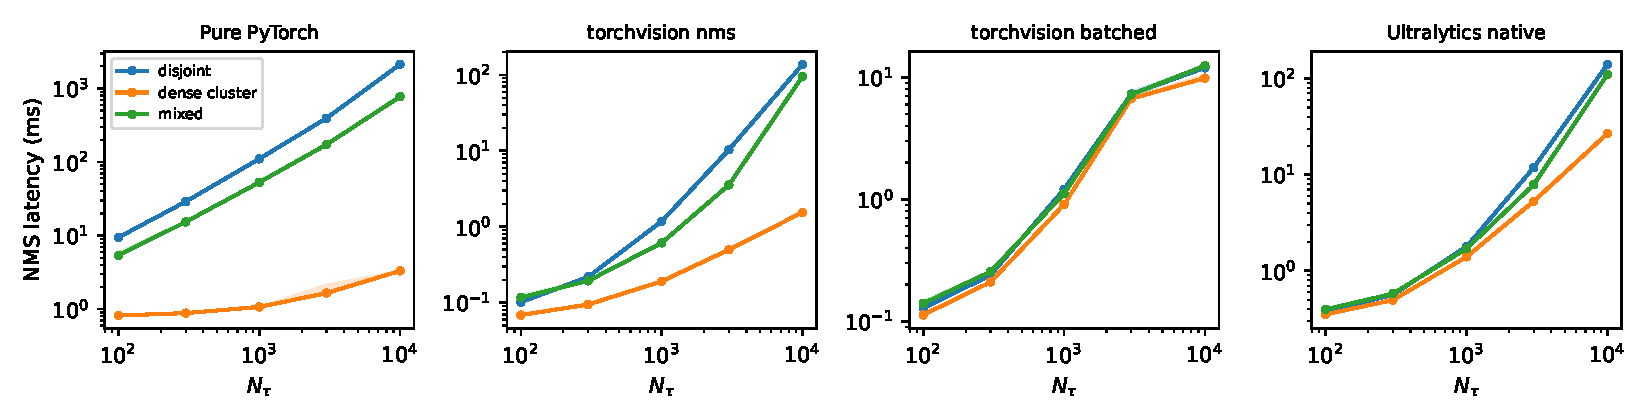
\includegraphics[width=0.9\textwidth]{fig2_dose_response.pdf}
\caption{Độ trễ NMS theo $\Ntau$ trên profile laptop đã ghim lõi (lưới 10\,000 anchor, 80 lớp, không giới hạn) cho bốn cách cài đặt và ba hình học hộp. Đường là trung vị; dải tô màu là khoảng tin cậy bootstrap 95\% theo các lần lặp. Cả hai trục đều là thang logarit.}
\label{fig:dose}
\end{figure*}

\subsection{Cách cài đặt, hình học, số lớp và giới hạn top-$k$}
\paragraph{Cách cài đặt và hình học ở cùng $\Ntau$ (H2).}
Tại $\Ntau=300$ trên head 2100 anchor với hình học hỗn hợp, NMS PyTorch thuần chậm hơn \texttt{nms} của torchvision 80 lần (tỷ số 80,3; khoảng tin cậy từ 76,4 đến 81,9), NMS gốc Ultralytics chậm hơn 2,9 lần (2,92; từ 2,79 đến 2,98), và \texttt{batched\_nms} của torchvision chậm hơn 1,3 lần (1,33; từ 1,24 đến 1,36). Hình học quan trọng không kém cách cài đặt. Tại $\Ntau=2100$, các hộp rời nhau tốn gấp 192 lần cụm dày đặc ở vòng lặp PyTorch thuần (khoảng tin cậy từ 189 đến 196), gấp 13 lần ở \texttt{nms} của torchvision (12,9 đến 14,7), gấp 1,8 lần ở cài đặt Ultralytics (1,74 đến 1,82), và không nhiều hơn ở \texttt{batched\_nms} của torchvision (1,01; từ 0,89 đến 1,07). Vì vậy ở cùng $\Ntau$, chi phí NMS có thể khác nhau hơn hai bậc độ lớn; đó là lý do cách cài đặt và hình học được báo cáo riêng xuyên suốt bài.

\paragraph{Tốc độ tăng mô tả.}
Bảng~\ref{tab:slopes} cho độ dốc của đường cong log--log trên $\Ntau\ge100$ với head 10\,000 anchor. Độ dốc gần một phù hợp với mức tăng tỷ lệ với $\Ntau$ và độ dốc lớn hơn một phù hợp với mức tăng nhanh hơn, nhưng chúng tôi không suy ra lớp độ phức tạp từ sáu mức; bảng chỉ mô tả đường cong đã đo. Đường cong cụm dày đặc của vòng lặp PyTorch thuần gần như phẳng (độ dốc 0,30), trong khi \texttt{nms} của torchvision trên các hộp rời nhau tăng với độ dốc 1,59.

\par\begin{center}
\centering\small
\captionof{table}{Độ dốc log--log của độ trễ NMS theo $\Ntau$ trên các mức đã đo $\ge 100$ (head 10\,000 anchor, 80 lớp, không giới hạn); khoảng tin cậy bootstrap 95\% trong ngoặc. Chỉ mang tính mô tả.}
\label{tab:slopes}
\begin{adjustbox}{max width=\columnwidth}
\begin{tabular}{@{}lccc@{}}
\toprule
Cách cài đặt & Rời nhau & Cụm dày đặc & Hỗn hợp \\
\midrule
PyTorch thuần & 1,17 [1,17; 1,17] & 0,30 [0,29; 0,32] & 1,07 [1,05; 1,08] \\
\texttt{nms} của torchvision & 1,59 [1,58; 1,60] & 0,69 [0,67; 0,69] & 1,42 [1,40; 1,45] \\
torchvision theo lô & 1,09 [1,08; 1,10] & 1,08 [1,07; 1,09] & 1,07 [1,05; 1,08] \\
Ultralytics gốc & 1,29 [1,29; 1,30] & 0,96 [0,95; 0,97] & 1,21 [1,20; 1,21] \\
\bottomrule
\end{tabular}
\end{adjustbox}
\end{center}\par

\paragraph{Số lớp.}
Các cài đặt không phân biệt lớp không bị ảnh hưởng bởi số lớp, đúng như kỳ vọng: tại $\Ntau=2100$ với hình học hỗn hợp, thời gian trung vị của NMS PyTorch thuần là 114,6~ms với 80 lớp và 116,5~ms với một lớp, còn của \texttt{nms} torchvision là 1,85 và 1,85~ms. Các cài đặt phân biệt lớp nhanh hơn khi chỉ có một lớp, vì các hộp thuộc lớp khác nhau không còn phải tách bằng phép dịch hoặc vòng lặp theo lớp: \texttt{batched\_nms} của torchvision mất 6,35~ms với 80 lớp và 2,16~ms với một lớp, và cài đặt Ultralytics lần lượt 4,45 và 2,39~ms. Do đó một bộ phát hiện phân biệt lớp có nhiều lớp thể hiện sự phụ thuộc vào $\Ntau$ khác với bộ phát hiện một lớp, và một phép so sánh chuẩn chỉ với một lớp sẽ đánh giá thấp sự phụ thuộc đó.

\paragraph{Giới hạn top-$k$ (H3).}
Bảng~\ref{tab:cap} và Hình~\ref{fig:cap} cho độ trễ NMS trung vị tại $\Ntau=10^4$ khi không có giới hạn và khi giới hạn 300 ứng viên. Giới hạn loại bỏ phần lớn chi phí: với các hộp rời nhau, vòng lặp PyTorch thuần giảm từ 2129 xuống 29,6~ms, \texttt{nms} của torchvision từ 137 xuống 0,21~ms, và cài đặt Ultralytics từ 140 xuống 0,54~ms. Việc chọn 300 điểm cao nhất thuộc công đoạn lọc điểm, vốn mất khoảng 0,29~ms tại $\Ntau=10^4$ khi không có giới hạn và 0,39~ms khi có giới hạn đối với nhánh PyTorch thuần. Một pipeline triển khai có giới hạn số ứng viên trước NMS sẽ chặn lợi ích mà việc tăng $\Ntau$ có thể mang lại, bất kể bộ tối ưu là gì.

\par\begin{center}
\centering\small
\captionof{table}{Độ trễ NMS trung vị (ms) tại $\Ntau=10^4$ (head 10\,000 anchor, 80 lớp) khi không có giới hạn và khi giới hạn 300 ứng viên.}
\label{tab:cap}
\begin{adjustbox}{max width=\columnwidth}
\begin{tabular}{@{}llcc@{}}
\toprule
Hình học & Cách cài đặt & Không giới hạn & Giới hạn 300 \\
\midrule
Rời nhau & PyTorch thuần & 2129 & 29,6 \\
 & \texttt{nms} của torchvision & 137 & 0,210 \\
 & torchvision theo lô & 12,0 & 0,244 \\
 & Ultralytics gốc & 140 & 0,542 \\
Hỗn hợp & PyTorch thuần & 775 & 15,2 \\
 & \texttt{nms} của torchvision & 95,4 & 0,184 \\
 & torchvision theo lô & 12,5 & 0,255 \\
 & Ultralytics gốc & 110 & 0,564 \\
Cụm dày đặc & PyTorch thuần & 3,31 & 0,904 \\
 & \texttt{nms} của torchvision & 1,54 & 0,102 \\
 & torchvision theo lô & 9,88 & 0,229 \\
 & Ultralytics gốc & 26,7 & 0,527 \\
\bottomrule
\end{tabular}
\end{adjustbox}
\end{center}\par

\begin{figure*}[!tp]
\centering
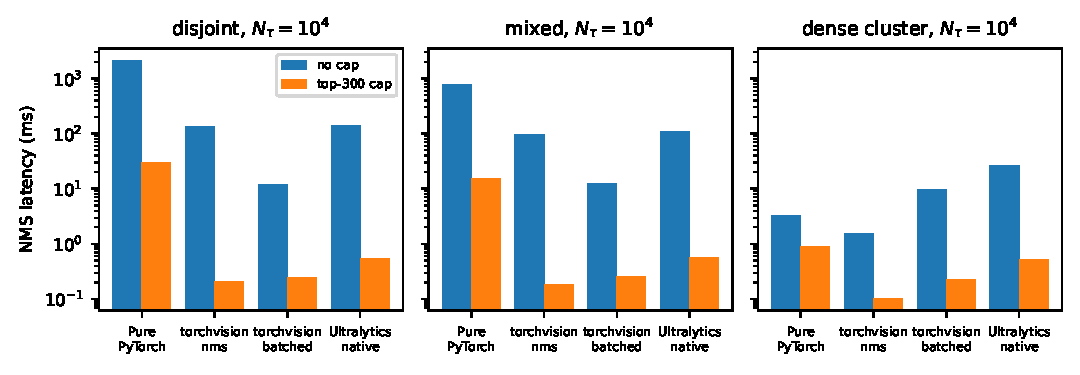
\includegraphics[width=0.9\textwidth]{fig5_cap_effect.pdf}
\caption{Độ trễ NMS trung vị tại $\Ntau=10^4$ (lưới 10\,000 anchor, 80 lớp) khi không giới hạn và khi giới hạn top-300, theo hình học và cách cài đặt; trục tung theo thang logarit.}
\label{fig:cap}
\end{figure*}

\subsection{Tiêm vào toàn bộ pipeline: cần bao nhiêu ứng viên để toàn trình chậm đi (H4)}
Để trả lời câu hỏi then chốt của bài ở mức toàn bộ pipeline, chúng tôi tiêm các tập ứng viên tổng hợp vào pipeline đầy đủ (lan truyền thuận thật trên ảnh, rồi lọc điểm và NMS) cho 20 ảnh giữ ra, bốn cách cài đặt, ba hình học, có và không có giới hạn top-300, ở 320 px ($\Ntau$ từ 0 đến 2100) và 640 px ($\Ntau$ từ 0 đến 8400). Ô $\Ntau=0$ của mỗi ảnh được đo ba lần ở ba vị trí ngẫu nhiên và dùng làm mẫu số. Với mỗi cách cài đặt và hình học, chúng tôi báo ngưỡng $N^{*}$: số ứng viên nhỏ nhất trong lưới đã đo mà tỷ số thời gian toàn trình so với $\Ntau=0$ có cận dưới khoảng tin cậy 95\% (bootstrap theo ảnh) vượt $1+\mathrm{MDE}$ của toàn trình (0,55\% ở 320 px, 1,9\% ở 640 px). Thiết kế, endpoint và quy tắc đọc được đăng ký trước. Việc ghim lõi qua kiểm chứng ở đầu và cuối phiên (số lõi hiệu dụng 0,97 và 0,83); 12 trong 21 điểm tham chiếu bị cờ drift (lệch lớn nhất 30\%) và được giữ trong phân tích.

Ngưỡng ở 640 px dùng MDE đã đăng ký trước (1,9\%, từ lần A/A 640 px đầu tiên); với MDE 0,69\% của lần A/A đo lại, các ngưỡng ở 640 px không đổi trừ một ô (torchvision theo lô, hình học hỗn hợp: 1000 thay vì 3000). Bảng~\ref{tab:nstar} và Hình~\ref{fig:nstar} cho kết quả. Với vòng lặp PyTorch thuần, toàn trình chậm đi rõ rệt từ 100 ứng viên ở 320 px và 300 ứng viên ở 640 px, và chậm 6,55 lần ở 2100 ứng viên (320 px), 10,9 lần ở 8400 ứng viên (640 px). Với các nhân thư viện, ngưỡng cao hơn nhiều và mức tăng nhỏ hơn: torchvision \texttt{nms} cần 1000 ứng viên ở 320 px (toàn trình tăng 1,11 lần ở 2100) và 3000 ứng viên ở 640 px (1,58 lần ở 8400); Ultralytics gốc cần 100 ứng viên ở 320 px nhưng chỉ tăng 1,15 lần ở 2100, và cần 3000 ứng viên ở 640 px. Với cụm dày đặc, nhiều ô không vượt ngưỡng ở 640 px. Giới hạn top-300 chặn hầu hết mức tăng: tại $\Ntau$ lớn nhất với hộp rời nhau, tỷ số toàn trình của torchvision \texttt{nms} và Ultralytics không vượt MDE ở cả hai độ phân giải, trong khi vòng lặp PyTorch thuần vẫn chậm 1,64 lần (320 px) và 1,20 lần (640 px), vì 300 hộp vẫn là nhiều với một vòng lặp Python. Để so sánh, patch thật tạo khoảng 90 ứng viên ở 320 px và 119 đến 138 ở 640 px (Mục~\ref{sec:casestudy}): thấp hơn mọi $N^{*}$ ở 640 px, và chỉ chạm biên $N^{*}=100$ của PyTorch thuần và Ultralytics ở 320 px. Vì $N^{*}$ lấy mức đầu tiên vượt ngưỡng trong một lưới thưa, nó nhạy với nhiễu ở các mức gần ngưỡng (ví dụ, PyTorch thuần với cụm dày đặc ở 320 px cho 1,067 ở 1000 ứng viên nhưng 1,022 ở 2100); bảng nên được đọc như bậc độ lớn của ngưỡng.

\begin{table*}[!tp]
\centering\small
\caption{Ngưỡng $N^{*}$ (số ứng viên nhỏ nhất trong lưới làm toàn trình tăng vượt MDE: 0,55\% ở 320 px, 1,9\% ở 640 px) theo cách cài đặt NMS và hình học, không giới hạn top-$k$; ``$>$'' nghĩa là không mức nào trong lưới vượt ngưỡng. Cột ``Tỷ số'' là tỷ số toàn trình ở $\Ntau$ lớn nhất với hộp rời nhau (2100 ở 320 px, 8400 ở 640 px). 20 ảnh, bootstrap theo ảnh.}
\label{tab:nstar}
\begin{adjustbox}{max width=\textwidth}
\begin{tabular}{@{}lcccccccc@{}}
\toprule
 & \multicolumn{4}{c}{320 px (lưới 100, 300, 1000, 2100)} & \multicolumn{4}{c}{640 px (lưới 300, 1000, 3000, 8400)} \\
\cmidrule(lr){2-5}\cmidrule(lr){6-9}
Cách cài đặt & Rời nhau & Hỗn hợp & Cụm dày đặc & Tỷ số & Rời nhau & Hỗn hợp & Cụm dày đặc & Tỷ số \\
\midrule
PyTorch thuần & 100 & 100 & 300 & 6,55 & 300 & 300 & $>$8400 & 10,9 \\
torchvision \texttt{nms} & 1000 & 1000 & 1000 & 1,11 & 3000 & 8400 & $>$8400 & 1,58 \\
torchvision theo lô & 300 & 1000 & 1000 & 1,21 & 1000 & 3000 & 3000 & 1,09 \\
Ultralytics gốc & 100 & 1000 & 1000 & 1,15 & 3000 & 3000 & 3000 & 1,59 \\
\bottomrule
\end{tabular}
\end{adjustbox}
\end{table*}

\begin{figure*}[!tp]
\centering
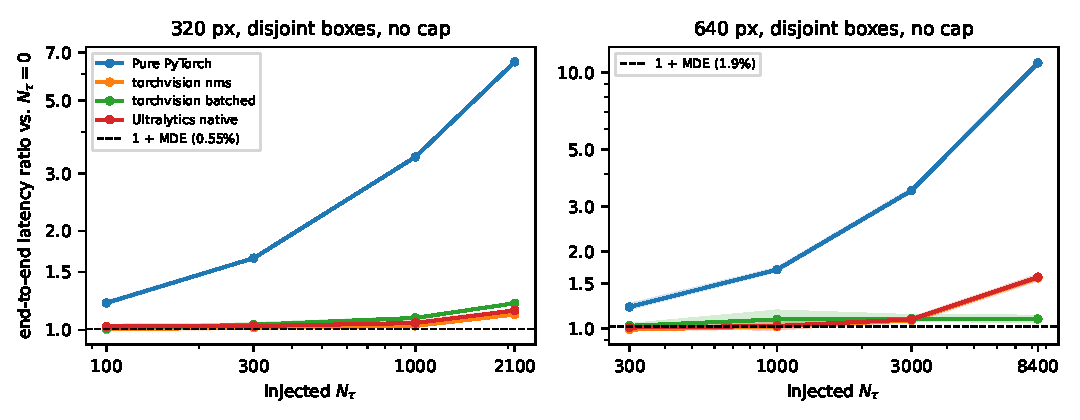
\includegraphics[width=0.9\textwidth]{fig4_pipeline_nstar.pdf}
\caption{Tỷ số thời gian toàn trình so với $\Ntau=0$ khi tiêm ứng viên rời nhau vào toàn bộ pipeline (20 ảnh, không giới hạn top-$k$), ở 320 px và 640 px. Đường nét đứt là $1+\mathrm{MDE}$ của toàn trình; dải mờ là khoảng tin cậy 95\% bootstrap theo ảnh. Cả hai trục theo thang logarit.}
\label{fig:nstar}
\end{figure*}

\paragraph{Mô hình Amdahl dự đoán ngưỡng $N^{*}$.}
Áp dụng mô hình ở Mục~\ref{sec:amdahl} với đường cong tiêm của đối chứng dương và thời gian toàn trình của ảnh sạch trong chính phiên này, tỷ số dự đoán khớp tỷ số đo trên 156 ô (bốn cách cài đặt, ba hình học, hai giới hạn, hai độ phân giải) với sai số log tuyệt đối trung vị 0,012 và phân vị 90 là 0,040 (Bảng~\ref{tab:amdahl_e9}). Ngưỡng dự đoán trùng đúng ngưỡng đo được ở 35 trên 48 ô; ở phần lớn các ô còn lại hai ngưỡng cách nhau một bậc của lưới, thường do các ô gần ngưỡng có khoảng tin cậy rộng. Phân tích này là post hoc, vì phép tiêm toàn pipeline đã được xem trước khi viết mô hình; phép kiểm tiến cứu nằm ở Mục~\ref{sec:attacks}.

\paragraph{Sàn nhiễu trong phiên và độ nhạy với drift.}
Từ ba ô $\Ntau=0$ của mỗi ảnh, sàn nhiễu ngay trong phiên (bản sao thứ hai so với bản sao thứ nhất) là 2,5--3,2\% ở 320 px và 3,3--6,3\% ở 640 px, cao hơn MDE của các lần A/A riêng (0,55\% và 0,69\%) vì mỗi ô chỉ có 3--5 lần lặp và các bản sao cách nhau về thời gian. Với sàn nhiễu này, các ngưỡng $N^{*}$ sẽ cao hơn những gì Bảng~\ref{tab:nstar} cho thấy; bảng giữ MDE đã đăng ký. Khi bỏ các khối có điểm tham chiếu bị cờ, phần lớn các ngưỡng không đổi.

\begin{table*}[!tp]
\centering\small
\caption{Mô hình Amdahl so với phép tiêm toàn pipeline (hộp rời nhau, không giới hạn): ngưỡng $N^{*}$ dự đoán và đo được, và tỷ số toàn trình dự đoán/đo ở $\Ntau$ lớn nhất.}
\label{tab:amdahl_e9}
\begin{adjustbox}{max width=\textwidth}
\begin{tabular}{@{}lcccc@{}}
\toprule
Cách cài đặt & $N^{*}$ dự đoán & $N^{*}$ đo & $R_{\mathrm{pred}}$ & $R_{\mathrm{meas}}$ \\
\midrule
\multicolumn{5}{@{}l}{\textit{320 px ($\Ntau=2100$)}} \\
PyTorch thuần & 100 & 100 & 6,44 & 6,57 \\
torchvision \texttt{nms} & 1000 & 1000 & 1,10 & 1,11 \\
torchvision theo lô & 1000 & 300 & 1,14 & 1,20 \\
Ultralytics gốc & 100 & 300 & 1,12 & 1,14 \\
\multicolumn{5}{@{}l}{\textit{640 px ($\Ntau=8400$)}} \\
PyTorch thuần & 300 & 300 & 10,5 & 10,9 \\
torchvision \texttt{nms} & 3000 & 3000 & 1,54 & 1,58 \\
torchvision theo lô & 3000 & 1000 & 1,06 & 1,09 \\
Ultralytics gốc & 3000 & 3000 & 1,56 & 1,59 \\
\bottomrule
\end{tabular}
\end{adjustbox}
\end{table*}

\subsection{Tấn công toàn ảnh thật: ứng viên tăng hàng trăm lần, toàn trình tăng 3\%}
\label{sec:attacks}
Bảng~\ref{tab:attacks} và Hình~\ref{fig:attacks} tóm tắt kết quả. Phiên đo các tấn công toàn ảnh qua kiểm chứng ghim lõi ở đầu và cuối (0,85 và 0,98) và không có điểm tham chiếu nào bị cờ (lệch tối đa 2\%). Các nhiễu loạn đẩy $\Ntau$ ở $\tau=0{,}25$ từ trung vị 45 ở ảnh sạch lên 5578,5 (Overload) và 4811,5 (Phantom Sponges), tức tỷ số trung bình 389 (khoảng tin cậy 135 đến 753) và 340 (104 đến 678); ở $\tau=0{,}01$, từ 254 lên khoảng 11\,700 và 14\,500. Công đoạn NMS tăng từ 0,05--0,35~ms lên 4,6--7,8~ms với các nhân thư viện và từ 0,52~ms lên 55--79~ms với vòng lặp PyTorch thuần. Tuy vậy, toàn trình với các nhân thư viện chỉ tăng từ khoảng 316~ms lên 324--328~ms: tỷ số 1,029 đến 1,034, với khoảng tin cậy loại trừ 1 (Bảng~\ref{tab:attacks}). Sàn nhiễu trong phiên là 2,0--2,4\%, nên mức tăng vượt sàn nhiễu ở torchvision \texttt{nms} nhưng chưa vượt ở hai nhân còn lại. Đây là cùng hiện tượng mà các biến thể này cho thấy trong dữ liệu lịch sử chưa ghim lõi (toàn trình tăng 2--6\% khi $\Ntau$ tăng khoảng 300 lần), nay được xác lập dưới giao thức có MDE.

Mô hình Amdahl, với đặc tả cố định trước khi đo, đạt quy tắc định trước ở 3 trên 6 ô: torchvision theo lô với cả hai tấn công (sai số trung vị 0,022 và 0,024) và torchvision \texttt{nms} với Phantom Sponges (0,031). Mô hình không đạt với torchvision \texttt{nms} và Overload (0,046; cận trên 0,058) và với Ultralytics ở cả hai tấn công, nơi nó dự đoán tỷ số 1,065--1,098 trong khi đo được 1,033. Có hai nguồn sai số. Thứ nhất, đường cong tổng hợp với hình học hỗn hợp đánh giá quá cao chi phí NMS của ứng viên thật: nội suy chỉ từ $\Ntau$ sai 1,6 đến 6 lần ở các tập ứng viên này (sai số log 0,47--1,78), vì ứng viên do tấn công sinh ra chồng lấn mạnh và bị loại nhanh. Thứ hai, ngay cả khi thay đường cong bằng thời gian NMS đo thật của chính tập ứng viên, mô hình chỉ có số hạng NMS vẫn hụt khoảng 2,5\% (sai số log 0,023--0,026), vì các công đoạn khác cũng tăng theo $\Ntau$ (lọc ngưỡng trên 25\,200 hàng và dựng đầu vào cho NMS). Mô hình đúng hơn phải cộng các công đoạn này và dùng một đường cong có hình học gần với ứng viên thật.

Áp dụng cùng biểu thức cho vòng lặp PyTorch thuần (không đo toàn trình vì chi phí) cho thấy điều gì sẽ xảy ra với một NMS chậm: 55--79~ms thêm vào khoảng 316~ms tương ứng mức tăng toàn trình khoảng 17--25\%. Và nếu lan truyền thuận nhanh hơn mười lần nhờ bộ tăng tốc trong khi NMS giữ nguyên trên CPU, mẫu số giảm xuống khoảng 30~ms và cùng mức tăng NMS của các nhân thư viện sẽ thành khoảng 15--25\% toàn trình. Đây là suy luận từ mô hình, chưa phải phép đo; nó cho thấy kết quả của bài gắn chặt với cấu hình CPU một lõi.

\begin{table*}[!tp]
\centering\small
\caption{Tấn công toàn ảnh thật (YOLOv5s, 640 px, 50 ảnh $\times$ 5 seed) dưới giao thức ghim lõi: tỷ số $\Ntau$ ($\tau=0{,}25$), tỷ số toàn trình đo được và dự đoán bởi mô hình Amdahl, sai số trung vị và kết luận theo quy tắc đăng ký trước (cận trên KTC $<0{,}05$). MDE trong phiên: 2,0\% (torchvision), 2,4\% (Ultralytics).}
\label{tab:attacks}
\begin{adjustbox}{max width=\textwidth}
\begin{tabular}{@{}llccccc@{}}
\toprule
Tấn công & Cách cài đặt & Tỷ số $\Ntau$ & $R_{\mathrm{meas}}$ (KTC 95\%) & $R_{\mathrm{pred}}$ & Sai số (KTC 95\%) & Quy tắc \\
\midrule
Overload & torchvision \texttt{nms} & 389 & 1,034 (1,022--1,045) & 1,067 & 0,046 (0,034--0,058) & không đạt \\
Overload & torchvision theo lô & 389 & 1,029 (1,017--1,041) & 1,027 & 0,022 (0,017--0,028) & đạt \\
Overload & Ultralytics gốc & 389 & 1,034 (1,022--1,047) & 1,098 & 0,067 (0,049--0,088) & không đạt \\
Phantom Sponges & torchvision \texttt{nms} & 340 & 1,032 (1,021--1,043) & 1,042 & 0,031 (0,024--0,038) & đạt \\
Phantom Sponges & torchvision theo lô & 340 & 1,031 (1,019--1,045) & 1,023 & 0,024 (0,019--0,030) & đạt \\
Phantom Sponges & Ultralytics gốc & 340 & 1,033 (1,020--1,046) & 1,065 & 0,044 (0,033--0,054) & không đạt \\
\bottomrule
\end{tabular}
\end{adjustbox}
\end{table*}

\begin{figure*}[!tp]
\centering
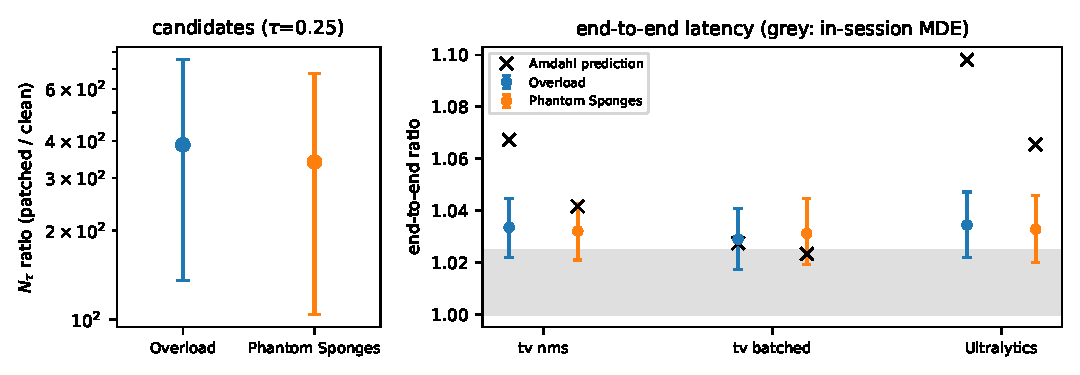
\includegraphics[width=0.9\textwidth]{fig9_attacks.pdf}
\caption{Tấn công toàn ảnh thật dưới giao thức ghim lõi (YOLOv5s, 640 px). Trái: tỷ số $\Ntau$ ($\tau=0{,}25$) so với ảnh sạch, thang logarit. Phải: tỷ số toàn trình đo được (điểm, khoảng tin cậy 95\%) và dự đoán của mô hình Amdahl đăng ký trước (dấu x) theo cách cài đặt NMS; dải xám là MDE trong phiên.}
\label{fig:attacks}
\end{figure*}

\subsection{Nghiên cứu tình huống: bộ tối ưu patch bằng thuật toán di truyền}
\label{sec:casestudy}
\paragraph{Bộ tối ưu.}
Bộ tối ưu của nghiên cứu tình huống đặt một patch ghi đè $64\times64$ tại cửa sổ có phương sai Laplacian lớn nhất của mỗi ảnh và tiến hóa các pixel của nó bằng thuật toán di truyền (quần thể 20, năm cá thể ưu tú, lai ghép tách ngang, đột biến Gauss) dưới EOT phần mềm. Hàm fitness là $\sum_i s_i \mathbb{1}[s_i>\tau]+\lambda \Ntau$ với $\lambda=1{,}5$, chỉ tính từ các điểm lớp trước NMS. Nó không chứa thành phần độ trễ nào và không dùng gradient. Đây chính là đại lượng mà quan hệ với độ trễ đang được nghiên cứu.

\paragraph{Quy mô.}
Các lần chạy trước đây tối ưu trên bốn ảnh. Ở đây tập tối ưu có 100 ảnh (một mẫu cố định, có seed, từ một tập con của tập huấn luyện COCO \cite{lin2014coco}), tách rời khỏi 100 ảnh giữ ra ngoài dùng để đo. Các điều kiện gồm: $320$ px với patch $64$ px ($4\%$ diện tích) tại $\tau=0{,}01$; $640$ px với patch $128$ px (cùng tỷ lệ diện tích); $320$ px với ngưỡng mục tiêu $\tau=0{,}25$; và, như một điều kiện phụ, $640$ px với patch $64$ px ($1\%$ diện tích). Mỗi điều kiện dùng mười seed tối ưu và cùng số lần đánh giá ứng viên như các lần chạy trước.

\paragraph{Các baseline.}
Chúng tôi đưa vào tìm kiếm ngẫu nhiên với đặt vị trí theo độ nổi bật, thuật toán di truyền với đặt vị trí ở tâm, thuật toán di truyền với đặt vị trí ngẫu nhiên, và một baseline leo gradient theo điểm số được điều chỉnh từ Overload \cite{overload2024}. Baseline gradient là một sự điều chỉnh cho patch ghi đè cục bộ và không phải một bản tái hiện của bản gốc.

\paragraph{Phép đo.}
Các patch được đóng băng bằng SHA-256 trước khi đo. Các ảnh giữ ra ngoài, có và không có mỗi patch, được đo trên profile đã ghim lõi: $\Ntau$ tại $\tau\in\{0{,}01;0{,}25\}$, các công đoạn lọc điểm và NMS cho bốn cách cài đặt, và độ trễ toàn trình cho hai cách cài đặt.

\paragraph{Kết quả tối ưu trên tập huấn luyện.}
Bảng~\ref{tab:train} và Hình~\ref{fig:budget} cho fitness huấn luyện tốt nhất đạt được ở mỗi mức ngân sách, lấy trung bình trên mười seed. Giá trị fitness phụ thuộc vào ngưỡng và kích thước đầu vào, nên có thể so sánh trong một nhóm cột cùng đầu vào và ngưỡng chứ không so được giữa các nhóm. Thuật toán di truyền bão hòa sớm: với C1, fitness tốt nhất trung bình tăng từ 185,1 ở 10\,000 lượt lên 186,6 ở 62\,500 lượt, tức tăng 0,8\%. Ở mức ngân sách cuối, tìm kiếm ngẫu nhiên với cùng cách đặt vị trí đạt 186,0, chỉ thấp hơn thuật toán di truyền 0,6, trong khi hai baseline đặt vị trí cao hơn (đặt ở tâm 191,0; đặt ngẫu nhiên 193,5), nên trên tập huấn luyện này lựa chọn vị trí đặt làm fitness thay đổi nhiều hơn quy trình tìm kiếm. Baseline gradient cao hơn xa mọi điều kiện không dùng gradient (334,1, giá trị ở bước cuối), đúng như kỳ vọng với một phương pháp hộp trắng dùng gradient của chính hàm mục tiêu. Thời gian đồng hồ trên GPU cho một seed và toàn bộ ngân sách là 30~s ở 320 px với các điều kiện không dùng gradient, 97 đến 98~s ở 640 px, và 86~s với baseline gradient.

\par\begin{center}
\centering\small
\captionof{table}{Fitness huấn luyện tốt nhất (trung bình trên mười seed, độ lệch chuẩn trong ngoặc) ở ba mức ngân sách (lượt lan truyền thuận ứng viên--ảnh). Với B4, giá trị là fitness ở bước cuối của mốc ngân sách, vì phương pháp gradient cập nhật một patch duy nhất và không giữ cá thể tốt nhất.}
\label{tab:train}
\begin{adjustbox}{max width=\columnwidth}
\begin{tabular}{@{}lccc@{}}
\toprule
Điều kiện & 10\,000 & 25\,000 & 62\,500 \\
\midrule
C1 (320 px, $\tau_{\mathrm{obj}}$ 0,01) & 185,1 (1,7) & 185,9 (1,2) & 186,6 (1,6) \\
C3 (320 px, $\tau_{\mathrm{obj}}$ 0,25) & 39,8 (0,2) & 40,0 (0,3) & 40,5 (0,3) \\
C2 (640 px, patch 128 px) & 294,4 (3,9) & 295,5 (2,9) & 297,3 (2,2) \\
C4 (640 px, patch 64 px) & 299,4 (1,3) & 301,4 (1,9) & 303,1 (1,7) \\
B1 (đặt ở tâm) & 188,7 (1,5) & 189,8 (1,0) & 191,0 (1,4) \\
B2 (đặt ngẫu nhiên) & 191,6 (1,9) & 193,1 (1,5) & 193,5 (1,9) \\
B3 (tìm kiếm ngẫu nhiên) & 184,5 (0,8) & 185,1 (0,8) & 186,0 (1,0) \\
B4 (gradient, tanh) & 218,1 (14,9) & 314,4 (12,8) & 334,1 (11,6) \\
\bottomrule
\end{tabular}
\end{adjustbox}
\end{center}\par

\par\begin{center}
\centering
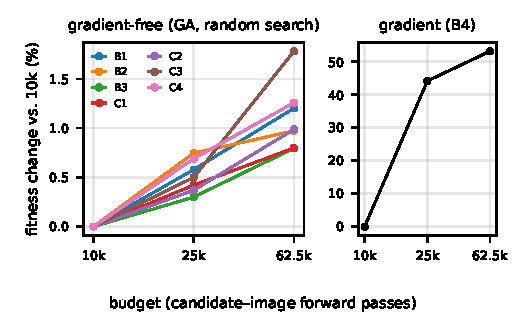
\includegraphics[width=\columnwidth]{fig7_training_budget.pdf}
\captionof{figure}{Thay đổi fitness huấn luyện (trung bình mười seed) theo ngân sách, so với mốc 10\,000 lượt. Khung trái (thang 0--2\%): các điều kiện không dùng gradient chỉ tăng dưới 2\%; khung phải (thang 0--60\%): baseline gradient B4 tăng khoảng 53\%.}
\label{fig:budget}
\end{center}\par

\paragraph{Kết quả đo lại.}
Các patch được sinh trên GPU, đóng băng bằng giá trị băm và đo trên profile laptop đã ghim lõi (số lõi hiệu dụng 0,84 dưới tải; 0 trên 11 điểm tham chiếu bị cờ drift; MDE toàn trình 0,55\%). Bảng~\ref{tab:patches} và Hình~\ref{fig:patches} cho tỷ số của ảnh có patch so với ảnh sạch ở 320 px. Có ba phát hiện đáng chú ý.

Thứ nhất, các patch của thuật toán di truyền không làm tăng $\Ntau$ một cách đo được: $\Ntau$ trung vị tại $\tau=0{,}01$ giảm từ 86,5 xuống 85,5 (320 px, $\tau_{\mathrm{obj}}=0{,}01$) và xuống 85 (320 px, $\tau_{\mathrm{obj}}=0{,}25$), và khoảng tin cậy của tỷ số trung bình chứa 1. Tìm kiếm ngẫu nhiên, GA đặt ở tâm và GA đặt vị trí ngẫu nhiên cho cùng một bức tranh. Thứ hai, tất cả chúng đều thêm một lượng thời gian toàn trình nhỏ nhưng đo được, từ 1,1 đến 1,5\%, với khoảng tin cậy loại trừ 1 nhưng ở mức khoảng gấp đôi MDE toàn trình; các baseline không dùng gradient cho cùng mức tăng, nên đây không phải đặc trưng của các patch đã tối ưu. Thứ ba, baseline gradient làm $\Ntau$ tăng 2,3 lần (trung vị từ 93 lên 166 tại $\tau=0{,}01$; 6,7 lần tại $\tau=0{,}25$) và làm công đoạn NMS của torchvision tăng 21\% và công đoạn NMS PyTorch thuần tăng 2,3 lần, nhưng tỷ số toàn trình của nó (gộp 100 ảnh) là 1,008 với khoảng tin cậy 95\% từ 1,002 đến 1,015, cận dưới chưa vượt $1+\mathrm{MDE}$. Dưới giao thức này, vì vậy, việc $\Ntau$ tăng 2,3 lần không nhìn thấy được ở mức toàn trình, bởi trên ảnh sạch NMS chỉ chiếm 0,16\% tổng thời gian (trung vị, profile torchvision) còn bước lan truyền thuận chiếm phần lớn.

Các điều kiện 640 px (patch 128 px chiếm 4\% diện tích, và 64 px chiếm 1\% diện tích) làm tăng $\Ntau$ tại $\tau=0{,}01$ từ 86,5 lên 134 và từ 93 lên 138,5 tương ứng. So với ảnh sạch 320 px, tỷ số thời gian của chúng là khoảng 3,5 đến 3,6, nhưng đó là chi phí của đầu vào lớn hơn chứ không phải của patch (tỷ số này khác tỷ số khoảng 3,4 suy từ Bảng~\ref{tab:aa} vì toàn trình của A/A gồm cả bước tải và đổi kích thước ảnh, còn phép đo patch bắt đầu từ tensor đã chuẩn bị, và hai phép đo ở hai phiên khác nhau). Vì thiết kế ban đầu không có nhánh sạch 640 px, chúng tôi bổ sung một lần đo đã đăng ký trước, trong đó ảnh sạch 640 px được đo cùng lượt với hai điều kiện patch 640 px. Lần đo bổ sung đầu tiên bị nhiễu nặng (một khối chậm 12 lần) và được đo lại với cùng mã; lần đo lại có số lõi hiệu dụng 0,94 và lệch tham chiếu tối đa 7,9\% (7 trong 11 điểm vượt cờ 3\%), và các số dưới đây lấy từ lần đo lại, so với MDE của lần A/A 640 px thứ hai (0,69\%). So với ảnh sạch 640 px (trung vị $\Ntau$ là 119 ở $\tau=0{,}01$), $\Ntau$ tăng lên 134 với patch 128 px (tỷ số 1,07; khoảng tin cậy 1,00 đến 1,16) và 138,5 với patch 64 px (1,07; 1,04 đến 1,10). Công đoạn NMS của torchvision tăng 1,9\% (0,99 đến 1,05) và 3,2\% (1,00 đến 1,07), công đoạn NMS PyTorch thuần tăng 10\% (1,02 đến 1,19) và 9\% (1,05 đến 1,14). Tỷ số toàn trình là 1,011 (1,005 đến 1,016) với torchvision và 1,008 (1,002 đến 1,014) với PyTorch thuần cho patch 128 px, và 1,012 (1,005 đến 1,019) và 1,014 (1,006 đến 1,022) cho patch 64 px. Các khoảng tin cậy loại trừ 1, nhưng cận dưới chưa vượt $1+\mathrm{MDE}$ (1,0069): mức tăng khoảng 1\%, cùng bậc với mức 1,1 đến 1,5\% đã thấy ở 320 px và cũng có ở các baseline không tối ưu.

\begin{table*}[!tp]
\centering\small
\caption{Tác động của các patch đã tối ưu so với ảnh sạch trên profile laptop đã ghim lõi. Tỷ số là có patch chia cho sạch; khoảng tin cậy là bootstrap hai tầng 95\% trên ảnh và seed; các cột NMS và toàn trình dùng pipeline torchvision; cột cuối là MDE A/A của công đoạn toàn trình. $^{\dagger}$So với ảnh sạch 640 px, lần đo bổ sung thứ hai; MDE từ lần A/A 640 px thứ hai. Mọi dòng dùng 100 ảnh $\times$ 5 seed (seed 0--4, chọn trước); với các baseline, ảnh 1--50 từ lần đo chính và ảnh 51--100 từ một lần đo bổ sung, mỗi ảnh so với ảnh sạch của chính phiên đo nó.}
\label{tab:patches}
\begin{adjustbox}{max width=\textwidth}
\begin{tabular}{@{}lccccc@{}}
\toprule
Điều kiện & Tỷ số $\Ntau$ ($\tau$=0,01) & Tỷ số $\Ntau$ ($\tau$=0,25) & Tỷ số độ trễ NMS & Tỷ số toàn trình & MDE (\%) \\
\midrule
320 px, 4\% diện tích, $\tau$=0,01 & 1,04 (0,99--1,10) & 0,94 (0,86--1,03) & 1,003 (0,987--1,018) & 1,013 (1,006--1,021) & 0,55 \\
320 px, 4\% diện tích, $\tau$=0,25 & 1,04 (0,99--1,09) & 0,95 (0,86--1,05) & 1,010 (0,992--1,028) & 1,015 (1,007--1,025) & 0,55 \\
640 px, 4\% diện tích, $\tau$=0,01$^{\dagger}$ & 1,07 (1,00--1,16) & 0,94 (0,89--0,99) & 1,019 (0,989--1,048) & 1,011 (1,005--1,016) & 0,69 \\
Tìm kiếm ngẫu nhiên & 1,03 (0,98--1,08) & 0,95 (0,86--1,07) & 1,006 (0,988--1,023) & 1,011 (1,003--1,019) & 0,55 \\
GA, đặt ở tâm & 1,05 (0,99--1,10) & 0,90 (0,83--0,99) & 1,017 (0,998--1,037) & 1,010 (1,002--1,020) & 0,55 \\
GA, đặt ngẫu nhiên & 1,06 (1,03--1,10) & 0,93 (0,87--0,97) & 1,022 (1,003--1,042) & 1,012 (1,005--1,022) & 0,55 \\
Leo gradient & 2,40 (2,09--2,74) & 6,8 (4,7--9,4) & 1,228 (1,197--1,260) & 1,008 (1,002--1,015) & 0,55 \\
\bottomrule
\end{tabular}
\end{adjustbox}
\end{table*}

\begin{figure*}[!tp]
\centering
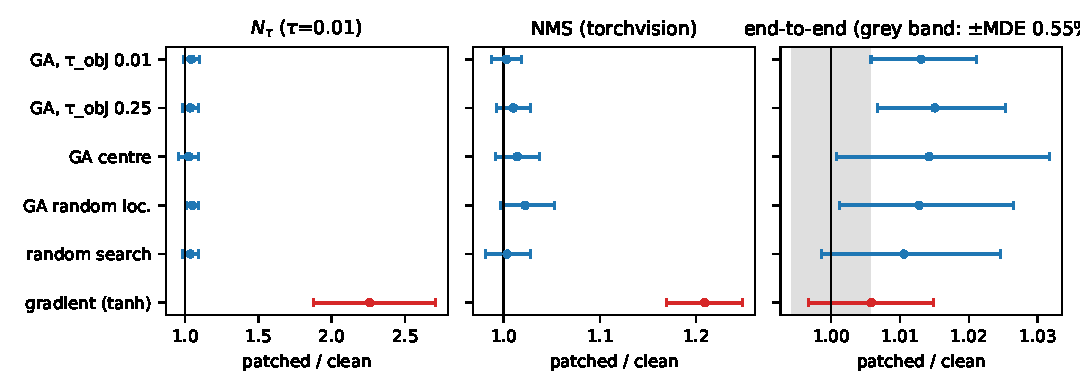
\includegraphics[width=0.9\textwidth]{fig6_patch_effects.pdf}
\caption{Tỷ số giữa ảnh có patch và ảnh sạch ở 320 px cho $\Ntau$, công đoạn NMS (torchvision) và toàn trình, với khoảng tin cậy 95\% bootstrap hai tầng. Dải xám ở khung phải là $\pm$MDE của toàn trình. Baseline gradient (đỏ) tăng $\Ntau$ và NMS rõ rệt nhưng toàn trình nằm trong dải MDE.}
\label{fig:patches}
\end{figure*}

\paragraph{Tác động lên từng cách cài đặt NMS.}
Bảng~\ref{tab:impl} phân rã các tỷ số công đoạn NMS của các điều kiện 320 px theo cách cài đặt. Các patch từ thuật toán di truyền (C1, C3) và các baseline tìm kiếm (B1--B3) giữ nguyên công đoạn NMS ở độ phân giải của giao thức, với hai ngoại lệ nằm trong mức nhiễu của nhiều phép so sánh: tỷ số PyTorch thuần của C1 (1,065; khoảng từ 1,003 đến 1,133) và của đặt ngẫu nhiên B2 (1,071; từ 1,021 đến 1,130) có khoảng tin cậy loại trừ 1. Baseline gradient B4 làm tăng công đoạn NMS ở mọi cách cài đặt: 2,29 với vòng lặp PyTorch thuần, 1,21 với \texttt{nms} của torchvision, và 1,11 với cả hai cài đặt phân biệt lớp. Tại $\tau=0{,}25$, các tỷ số PyTorch thuần và Ultralytics của B4 là 4,49 và 2,50. Như vậy công đoạn mà $\Ntau$ được cho là điều khiển có đáp ứng với mức tăng $\Ntau$ thật, và mức đáp ứng phụ thuộc vào cách cài đặt, đúng như các đường cong đáp ứng liều gợi ý.

\begin{table*}[!tp]
\centering\small
\caption{Tỷ số thời gian công đoạn NMS của ảnh có patch so với ảnh sạch tại $\tau=0{,}01$ (320 px; tỷ số trung bình, khoảng tin cậy bootstrap hai tầng 95\%). MDE A/A của công đoạn NMS là 0,64\% với vòng lặp PyTorch thuần và 1,1\% với \texttt{nms} của torchvision.}
\label{tab:impl}
\begin{adjustbox}{max width=\textwidth}
\begin{tabular}{@{}lcccc@{}}
\toprule
Điều kiện & PyTorch thuần & \texttt{nms} & Theo lô & Ultralytics \\
\midrule
C1 & 1,065 (1,003--1,133) & 1,003 (0,987--1,018) & 1,000 (0,987--1,013) & 1,006 (0,991--1,023) \\
C3 & 1,059 (0,997--1,126) & 1,010 (0,992--1,028) & 1,002 (0,987--1,018) & 1,004 (0,990--1,017) \\
B1 & 1,038 (0,965--1,114) & 1,014 (0,991--1,037) & 1,000 (0,983--1,017) & 0,995 (0,978--1,013) \\
B2 & 1,071 (1,021--1,130) & 1,022 (0,997--1,053) & 1,009 (0,993--1,028) & 1,005 (0,987--1,024) \\
B3 & 1,051 (0,975--1,131) & 1,003 (0,981--1,028) & 0,995 (0,978--1,013) & 0,993 (0,974--1,013) \\
B4 & 2,285 (1,894--2,735) & 1,209 (1,170--1,248) & 1,107 (1,083--1,131) & 1,107 (1,082--1,131) \\
\bottomrule
\end{tabular}
\end{adjustbox}
\end{table*}

\paragraph{NMS chiếm bao nhiêu trong pipeline?}
Trên ảnh sạch, công đoạn NMS của torchvision chiếm 0,16\% thời gian toàn trình (trung vị trên các ảnh); công đoạn NMS PyTorch thuần chiếm 2,4\% với ảnh của C1 và 2,9\% với ảnh của phép so sánh B4. Với baseline gradient, thời gian NMS tăng thêm bằng 0,034\% thời gian toàn trình của ảnh sạch (khoảng từ 0,028\% đến 0,040\%) với \texttt{nms} của torchvision, và 1,9\% (từ 1,5\% đến 2,3\%) với vòng lặp PyTorch thuần. Giá trị thứ nhất nhỏ hơn nhiều so với MDE toàn trình 0,55\% và giá trị thứ hai cùng bậc với nó, phù hợp với các tỷ số toàn trình 1,006 và 1,021 trong Bảng~\ref{tab:patches}. Pipeline bị chi phối bởi bước lan truyền thuận, và H4 giải thích lý do: với một bộ phát hiện nhỏ như YOLOv8n ở 320 px, bước lan truyền thuận mất khoảng 46~ms và ngay cả việc nhân đôi một công đoạn NMS nhanh cũng làm tổng thay đổi ít hơn mức mà giao thức phân giải được.

\paragraph{Các đánh giá trước đây của cùng bộ tối ưu.}
Trong các đánh giá trước đây, khi bộ tối ưu mới được tối ưu trên bốn ảnh và đánh giá trên 128 và sau đó 500 ảnh giữ ra (chưa có giao thức ghim lõi), SG-GA cũng không vượt GA đặt ở tâm: chênh lệch tỷ số ứng viên $-0{,}005$ (khoảng tin cậy từ $-0{,}011$ đến $0{,}001$) ở 128 ảnh và $-0{,}029$ (từ $-0{,}038$ đến $-0{,}022$; cả mười seed cùng dấu) ở 500 ảnh, trong đó tập 500 ảnh được mở rộng sau khi quan sát tập 128 ảnh và chứa nó. Các phân tích chi tiết của các đánh giá đó (diện tích, EOT, luồng dịch vụ, chuyển giao) không được dùng trong bài này.

\subsection{$\Ntau$ có dự đoán được độ trễ của các tập ứng viên thật không?}
Với mỗi đơn vị đo có $\Ntau>0$, chúng tôi dự đoán $t_{\mathrm{NMS}}$ chỉ từ $\Ntau$ bằng cách nội suy, trên thang log--log, đường cong đáp ứng liều của cách cài đặt và kích thước đầu vào tương ứng cho từng hình học. Chúng tôi báo cáo trung vị và phân vị 90 của $|\ln(t_{\mathrm{meas}}/t_{\mathrm{pred}})|$ so với đường cong hình học hỗn hợp và tỷ lệ các điểm đo nằm giữa đường cong rời nhau và đường cong cụm dày đặc. Các đại lượng này mô tả khoảng cách giữa dự đoán chỉ dựa trên $\Ntau$ và phép đo; không có ngưỡng đạt/không đạt nào được đặt trước.

Dự đoán chỉ dựa trên $\Ntau$ chính xác với một số cách cài đặt và kém với một số khác. Sai số log tuyệt đối trung vị so với đường cong hình học hỗn hợp là 0,05 với NMS gốc Ultralytics, 0,15 với NMS theo lô của torchvision, 0,33 với \texttt{nms} của torchvision, và 1,38 với PyTorch thuần, tức sai điển hình khoảng 4 lần với cài đặt sau; các phân vị 90 lần lượt là 0,15; 0,40; 0,47 và 1,73. Tỷ lệ trong 3347 điểm đo nằm giữa đường cong rời nhau và cụm dày đặc lần lượt là 0,44; 0,35; 0,93 và 0,76. Sai số xấp xỉ nhau giữa ảnh sạch và ảnh có patch (các nhánh ở Bảng~\ref{tab:patches}), nên chỗ sai là một tính chất của đường cong tổng hợp và các tập ứng viên thật chứ không phải của patch. Giữa các ảnh sạch, tương quan hạng của $\Ntau$ với thời gian NMS là cao (0,84 đến 0,94 tùy cách cài đặt), trong khi với sự thay đổi trong cùng một ảnh do patch gây ra nó thấp hơn (0,36 đến 0,73), gợi ý rằng $\Ntau$ xếp hạng chi phí giữa các ảnh tốt hơn là xếp hạng tác động của một chỉnh sửa lên một ảnh. Cả hai tương quan chỉ mang tính mô tả; các khoảng tin cậy 95\% có trong tệp tóm tắt.

\begin{figure*}[!tp]
\centering
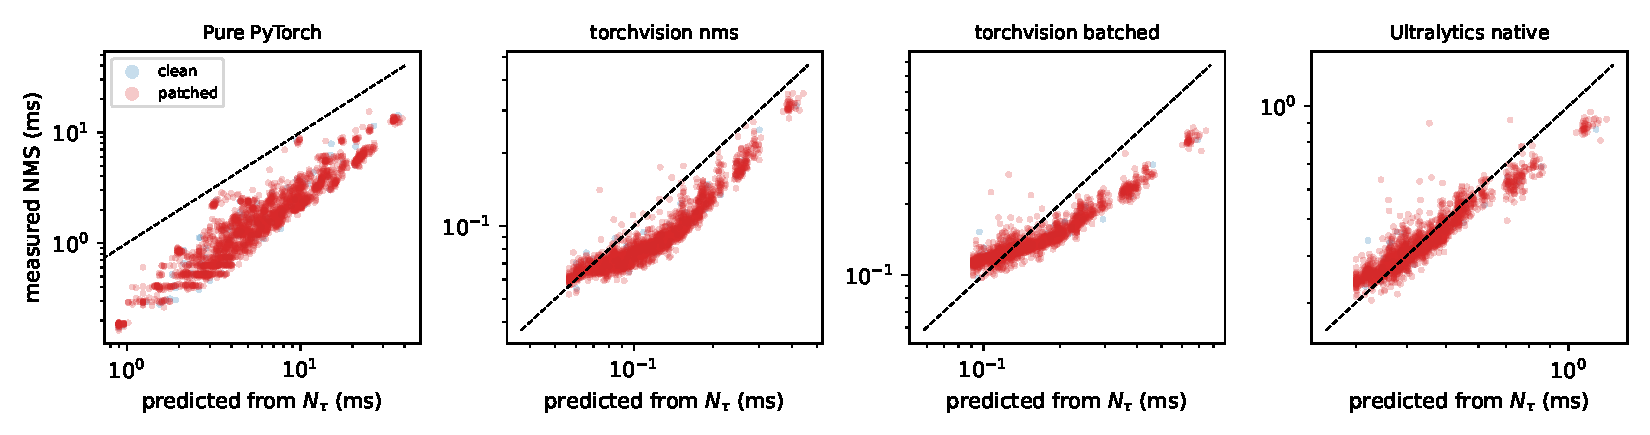
\includegraphics[width=0.9\textwidth]{fig3_pred_vs_measured.pdf}
\caption{Độ trễ NMS đo được của các tập ứng viên thật ($\tau=0{,}01$, các điều kiện 320 px) so với dự đoán chỉ dựa trên $\Ntau$ từ đường cong đáp ứng liều hình học hỗn hợp, theo từng cách cài đặt. Đường nét đứt là đường bằng nhau. Điểm xanh là ảnh sạch, điểm đỏ là ảnh có patch (các điểm sạch ít và phần lớn bị che vì mỗi ảnh sạch chỉ là một điểm).}
\label{fig:pred}
\end{figure*}

\subsection{Hình học có giải thích phần sai số còn lại không?}
\label{sec:nk}
Để định lượng phần mà hình học đóng góp, chúng tôi so hai mô hình log--tuyến tính khớp riêng cho từng cách cài đặt trên các ô của phép tiêm tổng hợp: $M_N$, $\ln t_{\mathrm{NMS}} = a + b\ln\Ntau$, và $M_{NK}$, thêm số hạng $c\ln\max(K,1)$ với $K$ là số hộp mà NMS giữ lại. $K$ là một đại diện cho hình học (rời nhau thì giữ gần hết, cụm dày đặc thì giữ ít), nhưng chỉ biết được sau khi chạy NMS, nên $M_{NK}$ là một phép phân rã chứ không phải một bộ dự đoán triển khai được. Đặc tả hai mô hình được cố định trước khi khớp; phép đánh giá xác nhận dùng các tập ứng viên thật ở 640 px (ảnh sạch 640 px và hai điều kiện patch 640 px), phép đánh giá ở 320 px được gắn nhãn post hoc vì sai số chỉ-từ-N trên tập này đã được xem trước. Lưu ý rằng $M_N$ là một đường hồi quy chung cho mọi hình học và số anchor, khác với phép nội suy theo đường cong hình học hỗn hợp ở mục trước, nên sai số của nó cao hơn.

Bảng~\ref{tab:nk} cho kết quả. Với vòng lặp PyTorch thuần, thêm $K$ làm sai số dự đoán giảm khoảng một nửa (ở 640 px, từ 0,90 xuống 0,45; chênh lệch 0,44 với khoảng tin cậy từ 0,28 đến 0,56), đúng như mô hình chi phí: thời gian của vòng lặp gần như tỷ lệ với số hộp được giữ lại. Với torchvision \texttt{nms}, không phát hiện cải thiện. Với hai cài đặt phân biệt lớp, $M_{NK}$ tệ hơn hẳn $M_N$ (ở 640 px, sai số từ 0,60 lên 1,79 với torchvision theo lô và từ 0,44 lên 2,16 với Ultralytics), và hệ số của $K$ âm ($-0{,}92$ và $-1{,}33$): mô hình học từ các tập tổng hợp, vốn gán 80 lớp ngẫu nhiên, ngoại suy sai sang các tập ứng viên thật có phân bố lớp khác hẳn. Ngay cả $M_N$ cũng lệch mức tuyệt đối ($R^2$ trên thang log âm ở ba trong bốn cài đặt). Hai kết quả cùng một chiều: $\Ntau$ một mình không đủ để dự đoán thời gian NMS, và một mô hình hiệu chuẩn hoàn toàn trên ứng viên tổng hợp không thay được phép đo trên ứng viên thật. Phép xác nhận theo đăng ký dùng lần đo patch 640 px đầu tiên (nhiễu cao); chạy lại trên lần đo thứ hai (ngoài đăng ký) cho cùng kết luận: thêm $K$ giảm sai số với PyTorch thuần (chênh lệch 0,69; 0,57 đến 0,81), không phát hiện cải thiện với torchvision \texttt{nms} (0,03; $-0{,}11$ đến 0,14), và làm sai số tệ hơn với hai cài đặt phân biệt lớp.

\par\begin{center}
\centering\small
\captionof{table}{Trung vị sai số $|\ln(t_{\mathrm{meas}}/t_{\mathrm{pred}})|$ của $M_N$ và $M_{NK}$ trên các tập ứng viên thật, và chênh lệch $\Delta$ (của $M_N$ trừ $M_{NK}$) với khoảng tin cậy 95\% bootstrap hai tầng (ảnh, đơn vị trong ảnh). $\Delta>0$ nghĩa là thêm $K$ làm giảm sai số.}
\label{tab:nk}
\begin{adjustbox}{max width=\columnwidth}
\begin{tabular}{@{}lccc@{}}
\toprule
Cách cài đặt & $M_N$ & $M_{NK}$ & $\Delta$ (KTC 95\%) \\
\midrule
\multicolumn{4}{@{}l}{\textit{640 px, đánh giá xác nhận (847 đơn vị, 100 ảnh)}} \\
PyTorch thuần & 0,90 & 0,45 & 0,44 (0,28 đến 0,56) \\
torchvision \texttt{nms} & 0,47 & 0,53 & $-0{,}07$ ($-0{,}21$ đến 0,04) \\
torchvision theo lô & 0,60 & 1,79 & $-1{,}19$ ($-1{,}34$ đến $-1{,}06$) \\
Ultralytics gốc & 0,44 & 2,16 & $-1{,}72$ ($-1{,}89$ đến $-1{,}52$) \\
\multicolumn{4}{@{}l}{\textit{320 px, post hoc (3347 đơn vị, 100 ảnh)}} \\
PyTorch thuần & 0,87 & 0,36 & 0,51 (0,40 đến 0,59) \\
torchvision \texttt{nms} & 0,44 & 0,50 & $-0{,}06$ ($-0{,}19$ đến 0,05) \\
torchvision theo lô & 0,53 & 1,87 & $-1{,}35$ ($-1{,}45$ đến $-1{,}22$) \\
Ultralytics gốc & 0,39 & 2,25 & $-1{,}86$ ($-1{,}96$ đến $-1{,}76$) \\
\bottomrule
\end{tabular}
\end{adjustbox}
\end{center}\par

\section{Thảo luận}
\label{sec:discussion}
\subsection{Mô hình Amdahl như một công cụ dự đoán}
Kết quả dương chính của bài là một quy tắc đơn giản, dùng được trước khi đo: tỷ số toàn trình xấp xỉ $1 + \Delta t_{\mathrm{NMS}}/t_{\mathrm{total}}$. Với ứng viên tổng hợp, quy tắc này dự đoán đúng tỷ số với sai số khoảng 1\% và dự đoán đúng ngưỡng $N^{*}$ ở phần lớn các ô; với tấn công thật, cấu trúc của quy tắc vẫn đứng nhưng hai đầu vào của nó phải chính xác hơn: chi phí NMS phải được đo hoặc mô hình hóa với hình học gần ứng viên thật, và các công đoạn khác phụ thuộc $\Ntau$ phải được cộng vào. Người đánh giá một tấn công độ trễ có thể dùng quy tắc này để biết trước một mức tăng $\Ntau$ có ý nghĩa ở thiết bị nào: chỉ cần tỷ phần NMS trên ảnh sạch và đường cong NMS của cách cài đặt đang dùng. Ngược lại, một khẳng định về độ trễ mà không nêu tỷ phần NMS và cách cài đặt không thể kiểm được.

\subsection{Đối chứng dương xác lập điều gì}
Giữa $10^2$ và $10^4$ ứng viên được tiêm, độ trễ NMS tăng từ 4 đến 1360 lần tùy cách cài đặt và hình học, và mức tăng được phát hiện ở MDE dưới 1,1\%. Vậy số ứng viên có ảnh hưởng đến thời gian NMS, nhưng mức ảnh hưởng phụ thuộc vào cách cài đặt NMS và vào cách các hộp chồng lấn; riêng $\Ntau$ không ấn định độ trễ. Kết quả vượt mốc (mọi lần lặp của pipeline PyTorch thuần với 2100 ứng viên đều vượt 100~ms) chỉ cho thấy bệ thử nghiệm có thể tạo ra một lần vượt mốc như vậy với cách cài đặt đó, không cho thấy một bộ phát hiện triển khai sẽ bị vượt mốc.

\subsection{Nghiên cứu tình huống bổ sung điều gì}
Hàm fitness của nghiên cứu tình huống không chứa thành phần độ trễ, nên mối liên hệ duy nhất của nó với độ trễ là giả định rằng $\Ntau$ theo sát độ trễ. Trong các phép đo của chúng tôi, câu trả lời là hỗn hợp. Giữa các ảnh, $\Ntau$ xếp hạng thời gian NMS tốt (tương quan hạng trên 0,84), và với baseline gradient thì thời gian NMS PyTorch thuần tăng 2,3 lần cùng với $\Ntau$. Tuy nhiên ở mức toàn bộ pipeline, cùng mức tăng 2,3 lần của $\Ntau$ làm thời gian toàn trình thay đổi ít hơn bề rộng khoảng tin cậy (1,008; khoảng 1,002 đến 1,015), vì bước lan truyền thuận chiếm phần lớn thời gian ở 320 px; các tấn công toàn ảnh đo lại dưới giao thức ghim lõi cho cùng kết luận ở quy mô lớn hơn nhiều ($\Ntau$ tăng khoảng 350 lần, toàn trình tăng khoảng 3\%). Các patch của thuật toán di truyền không làm tăng $\Ntau$ đo được, và mức tăng thời gian 1 đến 1,5\% của chúng cũng có ở tìm kiếm ngẫu nhiên và ở các baseline. Do đó chúng tôi không thấy bằng chứng nào ở đây cho thấy việc cực đại hóa $\Ntau$ bằng bộ tối ưu này tạo ra tác động độ trễ, và ở 640 px, so với ảnh sạch 640 px, toàn trình chỉ tăng khoảng 1\%, cận dưới chưa vượt MDE 0,69\%.

\subsection{Vì sao ứng viên không bảo đảm tăng độ trễ}
Chi phí NMS còn phụ thuộc phân bố hộp, mức chồng lấp, thứ tự điểm, cách cài đặt và giới hạn. Nhiều hộp bị loại nhanh có thể ít tốn hơn một tập nhỏ khó loại. Fitness thưởng ứng viên và điểm tin cậy nhưng chưa mô hình hóa trực tiếp những yếu tố này. Các tấn công toàn ảnh đo lại dưới giao thức ghim lõi minh họa trực tiếp: số ứng viên tăng khoảng 350 lần, công đoạn NMS tăng khoảng 20 đến 150 lần tùy cách cài đặt, nhưng toàn trình chỉ tăng khoảng 3\% vì NMS sau khi tăng vẫn chỉ chiếm khoảng 1,4 đến 2,3\% toàn trình. Một hàm mục tiêu độ trễ trực tiếp cũng không tự giải quyết vấn đề: bộ đếm thời gian chịu tiến trình nền, khởi động và backend. Nếu phát triển hàm mục tiêu quan sát độ trễ, cần cùng đường cơ sở, các khối ghép cặp ngẫu nhiên hóa, số lần đo lặp được tính vào ngân sách và một endpoint kiểm tra độc lập. Chưa thực hiện nhánh đó trong kết quả hiện tại, nên bài không báo hiệu lực hay cam kết cải thiện.

\subsection{Cơ chế}
Các phép đo phù hợp với mô hình chi phí ở Mục~\ref{sec:formal} ở bốn khía cạnh. Thứ nhất, độ trễ NMS có tăng theo $\Ntau$ (H1), với hệ số phụ thuộc cách cài đặt. Thứ hai, hình học quyết định mức tăng bao nhiêu (H2): cài đặt dùng vòng lặp dành gần như toàn bộ thời gian cho các hộp được giữ lại, nên các hộp rời nhau tốn hơn hai bậc độ lớn so với một cụm dày đặc cùng kích thước. Thứ ba, giới hạn chặn chi phí (H3): tại $\Ntau=10^4$, giới hạn 300 làm giảm thời gian PyTorch thuần trên hộp rời nhau 72 lần và thời gian torchvision 650 lần. Thứ tư, phần chiếm của NMS trong pipeline quyết định việc thay đổi ở công đoạn NMS có nhìn thấy ở mức toàn trình hay không (H4). Điều mà mô hình chi phí không cung cấp là cách đổi $\Ntau$ thành mili giây: dự đoán chỉ dựa trên $\Ntau$ sai gấp bốn lần với cài đặt dùng vòng lặp, dù chỉ sai khoảng 5\% với cài đặt Ultralytics.

\subsection{Vì sao bộ tối ưu của nghiên cứu tình huống không làm tăng $\Ntau$}
Fitness huấn luyện cho thấy thuật toán di truyền gần như không cải thiện so với tìm kiếm ngẫu nhiên (Bảng~\ref{tab:train}), và fitness của nó bị chi phối bởi vị trí đặt patch hơn là cách chọn các pixel; điều này nhất quán với các đánh giá trước đây của cùng bộ tối ưu, nơi SG-GA không khác tìm kiếm ngẫu nhiên và thấp hơn GA đặt ngẫu nhiên. Một patch 64 px phủ 4\% diện tích ảnh 320 px, và ngưỡng điểm 0,01 chấp nhận mọi anchor có chút bằng chứng về một đối tượng, nên số ứng viên chủ yếu do nội dung ảnh bên ngoài patch quyết định. Một phương pháp gradient bám theo gradient điểm số có thể nâng điểm của nhiều anchor cùng lúc và đạt số ứng viên gấp 2,3 lần; một tìm kiếm không dùng gradient với 625 lần đánh giá ứng viên không thể khám phá không gian đủ tốt. Đây là một quan sát về bộ tối ưu này và ngân sách này, không phải một phát biểu về tìm kiếm không gradient nói chung.

\subsection{Quan hệ với các khẳng định trong tài liệu}
Các mức tăng độ trễ được báo cáo của các tấn công NMS thường thu được với số lượng hộp lớn trên một nhân NMS dùng vòng lặp hoặc chạy trên GPU, trên một thiết bị biên cụ thể. Đối chứng dương của chúng tôi tái hiện khẳng định định tính trong một bối cảnh hẹp: với NMS dùng vòng lặp và hàng nghìn hộp rời nhau, độ trễ NMS tăng hai bậc độ lớn và thời gian toàn trình vượt mốc tham chiếu 100~ms. Cùng đối chứng đó cũng cho thấy bối cảnh này xa thực hành triển khai đến mức nào: với giới hạn 300 ứng viên, hiệu ứng giảm từ một đến ba bậc độ lớn, với một nhân thư viện phân biệt lớp thì giảm thêm, và với nội dung ảnh thực số ứng viên mà bộ tối ưu đạt được trên bộ phát hiện này thấp hơn số ứng viên được tiêm một đến hai bậc độ lớn (khoảng 90 so với $10^3$ đến $10^4$), trong khi các tấn công toàn ảnh hộp trắng đạt khoảng 5000 ứng viên nhưng chỉ làm toàn trình tăng khoảng 3\% trên CPU một lõi. Chúng tôi không đưa ra khẳng định nào về các bộ phát hiện hay thiết bị khác, và không kiểm tra các tấn công do các công trình được trích dẫn đề xuất. Kết quả của chúng tôi phù hợp với quan điểm rằng các tấn công độ trễ NMS cần một tổ hợp thuận lợi của cách cài đặt, giới hạn và hình học mới có ý nghĩa, một quan điểm mà EVADE lập luận từ một góc nhìn khác \cite{evade2025}.

\subsection{Hướng dẫn cho đánh giá và phòng thủ}
Với người đánh giá: báo cáo $\Ntau$ cùng cách cài đặt và giới hạn, đo từng công đoạn riêng, báo cáo sàn nhiễu A/A, và nêu mốc thời hạn nào đang được kiểm tra và vì sao. Với người phòng thủ: giới hạn số ứng viên trước NMS và một nhân thư viện có phân lô theo lớp là các thiết lập làm công đoạn NMS không nhạy với $\Ntau$ trong các phép đo của chúng tôi, và rẻ để áp dụng; bản thân việc chọn top-$k$ chỉ tốn một phần nhỏ của một mili giây. Giới hạn và ngưỡng cao hơn cũng có thể làm giảm độ chính xác, nên cấu hình hậu xử lý là một đánh đổi chứ không phải một bảo đảm. Với nhà nghiên cứu đề xuất một tấn công độ trễ: tối ưu độ trễ, hoặc một đại lượng thay thế mà quan hệ với độ trễ đã được kiểm chứng trên pipeline mục tiêu, và báo cáo hiệu ứng so với sàn nhiễu.

\subsection{Điều gì có thể làm đổi kết luận của chúng tôi}
Một bộ phát hiện lớn hơn trong đó NMS chiếm phần lớn hơn của pipeline, một độ phân giải khác (head thật ở 640 px có số anchor gấp bốn lần), một cách cài đặt có hằng số khác, hoặc một patch được tối ưu với thành phần độ trễ thay vì $\Ntau$ có thể tạo ra một tác động toàn trình mà nghiên cứu này không phát hiện được. Ở 640 px, mức tăng toàn trình khoảng 1\% nằm sát MDE (0,69\%); một thiết kế có nhiều ảnh hơn hoặc lặp nhiều hơn có thể đủ để phát hiện nó, nhưng độ lớn của nó vẫn nhỏ hơn nhiều so với chi phí của việc tăng độ phân giải.

\subsection{Đạo đức và dữ liệu}
Các phép thử chỉ xử lý dữ liệu và mô hình trong môi trường nghiên cứu được phép, không triển khai gây gián đoạn dịch vụ sản xuất. Chúng tôi tuân thủ điều khoản nguồn và quyền riêng tư; giấy phép của chú thích không tự cấp quyền tái phân phối mọi ảnh. Bộ công cụ đo, các manifest và các số đo cần thiết được công bố; chúng tôi không đóng gói patch tối ưu thành công cụ tấn công, vì không cần chúng để hỗ trợ luận điểm về giới hạn của đại lượng thay thế.

\section{Các mối đe dọa đối với tính hợp lệ}
\label{sec:threats}
\paragraph{Phạm vi thiết bị.}
Mọi phép đo đến từ một CPU laptop, suy luận float32 trên một lõi. Ở cấu hình này lan truyền thuận chiếm phần lớn thời gian (khoảng 46~ms ở 320 px, 166--180~ms ở 640 px với YOLOv8n, khoảng 316~ms với YOLOv5s), nên tỷ phần NMS nhỏ và theo mô hình Amdahl, mức tăng toàn trình bị nén lại. Các khẳng định của các tấn công độ trễ đã công bố đến từ GPU hoặc thiết bị biên có bộ tăng tốc, nơi tỷ phần NMS lớn hơn; bài này không đo các thiết bị đó, nên không bác bỏ các khẳng định đó mà chỉ cho công cụ để kiểm chúng. Một điện thoại Arm được chuẩn bị nhưng không qua kiểm chứng ghim lõi dưới tải, nên không có kết quả Arm.
\paragraph{Tính hợp lệ nội tại.}
Chế độ nguồn Windows Balanced được giữ nguyên nhưng tần số và turbo không bị khóa; luồng SMT anh em của lõi được ghim không bị chặn. Nhiễu thời gian được định lượng bằng A/A riêng (MDE toàn trình 0,55\% ở 320 px; ở 640 px lần A/A đầu bị nhiễu nặng với MDE 1,9\%, lần đo lại 0,69\%) và bằng sàn nhiễu trong phiên khi có thể (2,0--2,4\% ở phép đo tấn công toàn ảnh; 2,5--6,3\% ở phép tiêm toàn pipeline). Phép đo tham chiếu bị cờ drift ở 2/11 khối trong A/A 320 px, 2/12 trong đối chứng dương, 0/11 trong đo lại patch 320 px, 12/21 trong phép tiêm toàn pipeline (lớn nhất 30\%) và 0/11 trong phép đo tấn công toàn ảnh; các khối bị cờ được giữ, và các ngưỡng $N^{*}$ gần như không đổi khi bỏ chúng. Lần đo patch ở 640 px đầu tiên bị nhiễu nặng và được đo lại; bài dùng lần đo lại, chọn theo chất lượng phép đo chứ không theo giá trị tỷ số. Các ngưỡng $N^{*}$ ở 640 px dùng MDE đã đăng ký (1,9\%); với MDE 0,69\% của lần A/A đo lại, chúng không đổi trừ một ô. Mô hình Amdahl được viết sau khi xem phép tiêm toàn pipeline; chỉ phép kiểm trên tấn công toàn ảnh là tiến cứu. Patch được tối ưu trên 100 ảnh và đo trên 100 ảnh khác với năm trong mười seed tối ưu (0--4, chọn trước); mọi nhánh của bảng patch dùng 100 ảnh $\times$ 5 seed.
\paragraph{Tính hợp lệ cấu trúc.}
$\Ntau$ là số dự đoán vượt ngưỡng trước NMS. Độ trễ đo trên tensor đã chuẩn bị, không gồm giải mã ảnh, camera hay truyền tải. Mốc 100~ms là giá trị do nhóm chọn. Ứng viên tổng hợp có hình học được kiểm soát mà ứng viên thật không có; phép đo tấn công thật cho thấy hình học hỗn hợp tổng hợp đánh giá quá cao chi phí NMS. Giới hạn thời gian của hậu xử lý Ultralytics (2,05~s) không bị kích hoạt ở bất kỳ phép đo nào (thời gian NMS Ultralytics lớn nhất là khoảng 140~ms).
\paragraph{Tính hợp lệ bên ngoài.}
Hai bộ phát hiện một giai đoạn (YOLOv8n, YOLOv5s) và một họ dữ liệu (COCO). Các bộ phát hiện không NMS, mô hình lượng tử hóa và bộ tăng tốc không được bao phủ. Các tấn công toàn ảnh là biến thể đã điều chỉnh từ kho mã công khai, không phải tái hiện thí nghiệm gốc, và có quyền truy cập hộp trắng; patch được chèn dạng số, không có thử nghiệm in-và-chụp.
\paragraph{Tính hợp lệ của kết luận.}
Hiệu ứng được đọc so với MDE; khoảng tin cậy chứa một hoặc hiệu ứng dưới MDE được báo là không phát hiện ở độ nhạy đó, không phải tương đương. Các phân tích là ước lượng kèm khoảng tin cậy, không phải một họ kiểm định, nên không hiệu chỉnh đa phép thử.
\paragraph{Phạm vi của bộ tối ưu.}
Bộ tối ưu của nghiên cứu tình huống là hộp xám (đọc điểm trước NMS) và không tối thiểu hóa độ trễ trực tiếp. Bài không khẳng định một tấn công mạnh hơn các công trình trước, cũng không khẳng định một tấn công từ chối dịch vụ trên hệ thống triển khai nào.

\section{Kết luận và hướng phát triển}
\label{sec:conclusion}
Chúng tôi đã kiểm tra liệu số ứng viên trước NMS có dự đoán được độ trễ của bộ phát hiện không. Số ứng viên có ảnh hưởng đến thời gian NMS, nhưng mức ảnh hưởng phụ thuộc cách cài đặt và hình học tới hơn hai bậc độ lớn, và giới hạn top-$k$ chặn phần lớn. Ở mức toàn trình, một mô hình kiểu Amdahl không tham số khớp dự đoán tỷ số với sai số khoảng 1\% trên ứng viên tổng hợp, và cho biết cần bao nhiêu ứng viên để thấy toàn trình chậm đi. Trên các tấn công toàn ảnh thật đẩy $\Ntau$ lên khoảng 350 lần, toàn trình chỉ tăng khoảng 3\% trên CPU một lõi; mô hình đạt quy tắc định trước ở một nửa số ô và hụt vì đường cong tổng hợp đánh giá quá cao chi phí NMS của ứng viên thật và vì các công đoạn khác cũng tăng theo $\Ntau$. Một bộ tối ưu patch kiểu thuật toán di truyền không làm tăng $\Ntau$ và không vượt tìm kiếm ngẫu nhiên.

Hướng phát triển quan trọng nhất là đo cùng giao thức trên thiết bị có bộ tăng tốc (GPU, Jetson) và trên một thiết bị biên kiểm soát được (Raspberry Pi 5), nơi mô hình dự đoán tỷ phần NMS lớn hơn nhiều, và với tần số CPU được khóa; tiếp theo là bổ sung vào mô hình các công đoạn phụ thuộc $\Ntau$ ngoài NMS và một đường cong hình học sát ứng viên thật.

\FloatBarrier
\section*{Phát hành có trách nhiệm}
Các sản phẩm được phát hành là bộ công cụ đo, các manifest, các fixture tiêm tổng hợp và các bản ghi thời gian thô. Các patch đã tối ưu không được đóng gói thành công cụ, và công việc giới hạn trong một bệ thử nghiệm cục bộ.

\section*{Sẵn có dữ liệu và mã}
Mã, các manifest kèm giá trị băm tệp và các bản ghi thời gian thô nằm trong kho mã của dự án \url{https://github.com/reikageisme/Sponge-patch-nms}. Kho chứa các tệp đăng ký trước cùng các tag quản lý phiên bản, bộ công cụ và các script phân tích, các manifest (ghi mã băm, phiên bản thư viện, cấu trúc CPU và chế độ nguồn), giá trị băm của mọi patch, các bản ghi thời gian thô của mọi lần chạy kể cả các lần bị loại, và các script sinh hình. Mọi con số trong các bảng truy được tới một selector trong tệp tóm tắt do một script trong kho tạo ra (Phụ lục~\ref{app:src}).

\section*{Tuyên bố sử dụng AI tạo sinh}
Một trợ lý lập trình AI (Claude Code) đã được dùng để giúp viết và kiểm thử bộ công cụ đo và để soạn thảo các phần của bản thảo. Các tác giả đặt giả thuyết và endpoint, chạy các phép đo, đối chiếu mọi con số được báo cáo với bản ghi thô, và chịu trách nhiệm về nội dung.

\section*{Tài trợ, lời cảm ơn và xung đột lợi ích}
\paragraph{Tài trợ.} Nghiên cứu này không nhận tài trợ bên ngoài; đây là một dự án nghiên cứu độc lập của các tác giả.
\paragraph{Lời cảm ơn.} Nhóm cảm ơn giảng viên Đinh Phương Nam, Trường Đại học Công nghệ Thành phố Hồ Chí Minh (HUTECH), đã hướng dẫn thực hiện đề tài và phản biện cách diễn giải số liệu, các đường cơ sở và lợi ích của hướng nghiên cứu.
\paragraph{Tuyên bố về xung đột lợi ích.} Các tác giả tuyên bố không có xung đột lợi ích.

\appendix
\section{Nguồn số liệu}
\label{app:src}
Mọi con số trong bài truy được tới một trường trong tệp tóm tắt do một script trong kho mã tạo ra. Bảng đối chiếu từng nhóm số với tệp nguồn và trạng thái truy vết (đã kiểm lại hay còn phải truy lại) nằm trong tệp \texttt{docs/NGUON\_SO\_LIEU.md} của kho mã, không đưa đường dẫn vào thân bài.

\bibliographystyle{unsrtnat}
\bibliography{references}

\end{document}
